\documentclass[]{article}

\usepackage{amssymb}
\usepackage{amsmath}

\usepackage[headings]{fullpage}

\usepackage{caption}
\usepackage{subcaption}
\usepackage{graphicx}
\usepackage{float}

%settings voor listing
\usepackage{listings}
\lstset{
	 basicstyle=\footnotesize,
	 frame=single,
	 tabsize=2
}

%header en footer
\usepackage{fancyhdr}
\pagestyle{fancy}
\rhead{\tiny Vakoverschrijdend Project}
\lhead{\tiny Team Edran}
\lfoot{\tiny \today}

\usepackage{titlesec}
\titleformat{\part}[hang] 
{\normalfont\Large\bfseries}{Deel \thepart:}{0.5em} 
{}
\begin{document}
\tableofcontents

\setcounter{section}{0}
\setcounter{subsection}{0}
\section{Usecases}
\part{Het reserveren van ritten en goedkeuren/afkeuren van reservaties (ep I)}

\subsection{Auto + tijdstip bekijken}
\begin{itemize}
\item \textbf{Precondities:} autolener is ingelogd
\item \textbf{Trigger:} autolener bekijkt kalender
\item \textbf{Acties:} \begin{itemize}
\item	autolener zoekt op basis van tijdstip, naam auto, capaciteit auto, geografische standplaats
\item	systeem geeft meest passende mogelijke reservaties eerst terug
\item	autolener kiest auto + tijdstip 
\item 	systeem geeft details reservatie terug (naam auto, tijdstip, capaciteit, standplaats) + de naburige autoleners hun naam, telefoonnummer en emailadres
\end{itemize}
\item \textbf{Postcondities:} auto + tijdstip weergegeven
\end{itemize}


\subsection{Auto reserveren} \label{reserveren}
\begin{itemize}
\item \textbf{Precondities:} autolener is ingelogd, autolener bekijkt auto + tijdstip
\item \textbf{Trigger:} autolener kiest reserveren
\item \textbf{Acties:} \begin{itemize}
\item 	autolener geeft duur aan van de reservatie
\item systeem controleert of auto beschikbaar is voor deze duur
\item systeem slaat reservatie op in DB
\item      systeem laat autolener weten dat reservatie is gelukt
\item      systeem informeert eigenaar van de reservatie zodat deze die kan afhandelen
\end{itemize}
\item \textbf{Postcondities:} reservatie is toestand 'aanvraag'
\end{itemize}


\subsection{Eigenaar keurt reservatie goed}
\begin{itemize}
\item \textbf{Precondities:} eigenaar is ingelogd en bekijkt zijn reservatie-aanvragen \item \textbf{Trigger:} eigenaar kiest bepaalde reservatie
\item \textbf{Acties:} \begin{itemize}
\item	eigenaar kiest goedkeuren
	
\item	systeem slaat reservatie op in DB
\item      systeem laat eigenaar weten dat goedkeuren is gelukt
\item      systeem informeert autolener van de goedkeuring
\end{itemize}
\item \textbf{Postcondities:} reservatie is toestand 'goedgekeurd'
\end{itemize}


\subsection{Eigenaar weigert reservatie}
\begin{itemize}
\item \textbf{Precondities:} eigenaar is ingelogd en bekijkt zijn reservatie-aanvragen \item \textbf{Trigger:} eigenaar kiest bepaalde reservatie
\item \textbf{Acties:} \begin{itemize}
\item	eigenaar kiest weigeren
\item	eigenaar voegt korte reden toe voor weigering
\item	systeem slaat reservatie op in DB
\item      systeem laat eigenaar weten dat weigeren is gelukt
\item      systeem informeert autolener van de weigering
\end{itemize}
\item \textbf{Postcondities:} reservatie is toestand 'geweigerd'
\end{itemize}

\subsection{Autolener annuleert reservatie}
\begin{itemize}
\item \textbf{Precondities:} autolener is ingelogd en bekijkt zijn reservaties \item \textbf{Trigger:} autolener kiest bepaalde reservatie
\item \textbf{Acties:} \begin{itemize}
\item	eigenaar kiest annuleren
\item	systeem slaat reservatie op in DB
\item      systeem laat autolener weten dat annuleren is gelukt
\item      systeem informeert eigenaar van de annulatie
\end{itemize}
\item \textbf{Postcondities:} reservatie is toestand 'geannuleerd'
\end{itemize}

\subsection{Autolener verkort reservatie}
\begin{itemize}
\item \textbf{Precondities:} autolener is ingelogd en bekijkt zijn reservaties \item \textbf{Trigger:} autolener kiest bepaalde reservatie
\item \textbf{Acties:} \begin{itemize}
\item	autolener kiest inkorten
\item	autolener kiest nieuwe duur
\item	systeem controleert of auto beschikbaar is voor deze duur
\item	systeem slaat reservatie op in DB
\item      systeem laat autolener weten dat inkorten is gelukt
\item      systeem informeert eigenaar van de inkorting
\end{itemize}
\item \textbf{Postcondities:} reservatie is ingekort
\end{itemize}

\subsection{Eigenaar reserveert eigen auto}
\begin{itemize}
\item \textbf{Precondities:} eigenaar is ingelogd, eigenaar bekijkt zijn eigen auto
\item \textbf{Trigger:} eigenaar kiest tijdstip
\item \textbf{Acties:} \begin{itemize}
\item	eigenaar kiest reserveren
\item 	eigenaar kiest duur reservatie
\item	systeem controleert of auto beschikbaar is voor deze duur
\item	systeem slaat reservatie op in DB
\item      systeem laat eigenaar weten dat reservatie is gelukt
\end{itemize}
\item \textbf{Postcondities:} reservatie is toestand 'goedgekeurd'
\end{itemize}

\part{Registeren voor infosessie (ep I)}

\subsection{Inschrijven infosessie}
\begin{itemize}

\item \textbf{Precondities:} gewone gebruiker is ingelogd
\item \textbf{Trigger:} gebruiker kiest een bepaalde infosessie op de kalender of op een aparte pagina voor infosessies 
\item \textbf{Acties:} \begin{itemize}
\item	gebruiker kiest inschrijven
\item	de gebruiker krijgt een bericht van het systeem dat de inschrijving is gelukt
\item	het systeem voegt de gebruiker toe aan een lijst van aanwezigen bij een bepaalde infosessie
\end{itemize}
\item \textbf{Postcondities:} De gebruiker krijgt de toestand \emph{aanwezig/ingeschreven}.
\end{itemize}

\subsection{Uitschrijven infosessie}
\begin{itemize}

\item \textbf{Precondities:} gewone gebruiker is ingelogd
\item \textbf{Trigger:} gebruiker kiest een bepaalde infosessie op de kalender waarvoor hij op aanwezig staat 
\item \textbf{Acties:} \begin{itemize}
\item	gebruiker kiest uitschrijven
\item	de gebruiker krijgt een bericht van het systeem dat de uitschrijving is gelukt
\item	het systeem verwijdert de gebruiker van de lijst van aanwezigen bij een bepaalde infosessie
\end{itemize}
\item \textbf{Postcondities:} De gebruiker krijgt de toestand \emph{afwezig}.
\end{itemize}


\subsection{Infosessie aanmaken}
\begin{itemize}
\item \textbf{Precondities:} beheerder is ingelogd en bekijkt infosessies
\item \textbf{Trigger:} beheerder kiest nieuwe infosessie aanmaken
\item \textbf{Acties:} \begin{itemize}
\item	beheerder geeft datum, tijdstip, locatie en beschrijving nieuwe infosessie in
\item 	systeem slaat dit op in DB
\item	systeem laat weten aan beheerder dat de infosessie in aangemaakt
\end{itemize}
\item \textbf{Postcondities:} infosessie aangemaakt
\end{itemize}

\subsection{Details infosessie bekijken}
\begin{itemize}
\item \textbf{Precondities:} beheerder is ingelogd en bekijkt infosessies
\item \textbf{Trigger:} beheerder kiest bepaalde infosessie
\item \textbf{Acties:} \begin{itemize}
\item	beheerder kiest om details te bekijken
\item 	systeem geeft lijst van deelnemers, hun status binnen de groep en of ze zijn komen opdagen weer
\end{itemize}
\item \textbf{Postcondities:} details infosessie weergegeven
\end{itemize}

\subsection{Een aanwezigheidslijst van een infosessie invoeren}
\begin{itemize}
\item \textbf{Precondities:} Een beheerder met de machtiging om infosessies aan te passen of aan te maken is ingelogd op het systeem.
\item \textbf{Trigger:} de beheerder bekijkt de beheerspagina van een infosessie nadat de infosessie geweest is.
\item \textbf{Acties:} 
\begin{itemize}
	\item	De beheerder selecteert de gebruikers die op aanwezig stonden, maar toch afwezig waren en past dit aan.
	\item	Het systeem promoveert de aanwezige gebruikers tot \emph{aanwezig} en de afwezige gebruikers tot \emph{niet opgedaagd}. De laatsten krijgen dan een kans om zich voor een nieuwe infosessie in te schrijven.
\end{itemize}
\item \textbf{Postcondities:} De promoties na een infosessie zijn doorgevoerd in het systeem; de infosessie wordt afgesloten (geen bewerkingen meer mogelijk).
\end{itemize}

\part{Editeerbare emails versturen door het systeem (ep I)}

\subsection{Een beheerder past een standaard-mail aan}
\begin{itemize}
\item \textbf{Precondities:} een beheerder met de machtiging om mails aan te passen en te versturen is ingelogd op het systeem.
\item \textbf{Trigger:} de beheerder selecteert om een bepaald standaard-mail aan te passen.
\item \textbf{Acties:} 
\begin{itemize}
	\item	Het systeem toont een editor aan de beheerder met hierin de huidige HTML-code (+ SCALA-code) van de mail.
	\item	De beheerder voert de gewenste wijzigingen uit.
	\item	Het systeem verifi\"{e}ert de correctheid van de nieuwe code.
		\begin{itemize}
			\item Indien de verificatie mislukt, worden de fouten afgeprint en moet de gebruiker de fouten eerst herstellen.
		\end{itemize}
\end{itemize}
\item \textbf{Postcondities:} Indien de verificatie lukt, is de code van de standaard-mail aangepast.
\end{itemize}

\subsection{Een beheerder stuurt een standaard-email naar een gebruiker}
\begin{itemize}
\item \textbf{Precondities:} een beheerder met de machtiging om mails aan te passen en te versturen is ingelogd op het systeem.
\item \textbf{Trigger:} de beheerder selecteert om een bepaald standaard-mail te versturen
\item \textbf{Acties:} 
\begin{itemize}
	\item	De beheerder selecteert een gebruiker of meerdere gebruikers (een volledige autogroep, alle gebruikers binnen een bepaalde regio, ...).
	\item	De beheerder selecteert \emph{versturen}.
\end{itemize}
\item \textbf{Postcondities:} Het systeem verstuurt een email naar de geselecteerde gebruikers.
\end{itemize}

\subsection{Het systeem verstuurt een notificatiemail naar een gebruiker}
\begin{itemize}
\item \textbf{Precondities:} /
\item \textbf{Trigger:} een event waarvoor een notificatiemail verstuurt moet worden doet zich voor (bijvoorbeeld: een gebruiker heeft 3 of meer openstaande ritten waarvan de ritgegevens ingevuld moeten worden).
\item \textbf{Acties:} 
\begin{itemize}
	\item	Het systeem verstuurt de notificatiemail horende bij het event.
\end{itemize}
\item \textbf{Postcondities:} De gebruiker ontvangt een notificatiemail.
\end{itemize}

\part{Inloggen, registreren en wachtwoord vergeten (ep II)}
\subsection{Nieuwe autolener registreert zich}
\begin{itemize}
\item \textbf{Precondities:} nieuwe autolener is op website
\item \textbf{Trigger:} nieuwe autolener kiest registreren
\item \textbf{Acties:} \begin{itemize}
\item	autolener geeft zijn naam, voornaam, adres, postcode, stad, telefoonnummer in
\item autolener geeft emailadres en wachtwoord 2 keer in
\item autolener geeft eerste en tweede keuze voor infosessie in
\item	systeem controleert of emailadres uniek is 
\item systeem slaat autolener op in DB
\item systeem verzend wachtwoord via email naar autolener
\item      systeem laat autolener weten dat registratie is gelukt
\item      Include: inloggen, zie \ref{inloggen}
\end{itemize}
\item \textbf{Postcondities:} autolener is geregistreerd en is in toestand "ingeschreven" + is ingelogd
\end{itemize}

\subsection{Gebruiker logt in} \label{inloggen}
\begin{itemize}
\item \textbf{Precondities:} gebruiker is op website
\item \textbf{Trigger:} gebruiker kiest inloggen
\item \textbf{Acties:} \begin{itemize}
\item	gebruiker geeft email en wachtwoord in
\item	systeem controleert of emailadres en wachtwoord klopt
\item 	systeem logt gebruiker in
\item      systeem laat gebruiker weten dat inloggen is gelukt
\end{itemize}
\item \textbf{Postcondities:} gebruiker is ingelogd
\end{itemize}

\subsection{Nieuwe autoeigenaar registreert zich}
\begin{itemize}
\item \textbf{Precondities:} nieuwe eigenaar is op website
\item \textbf{Trigger:} nieuwe eigenaar kiest registreren
\item \textbf{Acties:} \begin{itemize}
\item	eigenaar geeft zijn naam, voornaam, adres, postcode, stad, telefoonnummer in
\item	eigenaar geeft zijn email en wachtwoord 2 keer in
\item	eigenaar geeft zijn automerk, model, bouwjaar, brandstof, jaarlijkse kilometers, huidige kilometerstand, naam verzekering, vervaldatum polis, polisnummer, bonus-malus, aantal zitplaatsen, trekhaak, GPS, gemiddelde verbruik per kilometer, huidige geschatte waarde, nummerplaat, volume koffer, inschrijvingsbewijs, chassisnummer en verschillende foto's in
\item	eigenaar geeft optionele commentaar bij de auto
\item eigenaar geeft uniek emailadres in 
\item	systeem controleert of emailadres uniek is 
\item systeem slaat eigenaar op in DB
\item systeem verzend wachtwoord via email naar eigenaar
\item      systeem laat eigenaar weten dat registratie is gelukt
\item      Include: inloggen, zie \ref{inloggen}
\end{itemize}
\item \textbf{Postcondities:} eigenaar is geregistreerd en is in toestand "ingeschreven" + is ingelogd
\end{itemize}

\subsection{Nieuwe autolener/autobeheerder vervolledigt registratie}
\begin{itemize}
\item \textbf{Precondities:} nieuwe autolener/autobeheerder is ingelogd en heeft toestand aanwezig
\item \textbf{Trigger:} nieuwe autolener/autobeheerder kiest registratie voltooien
\item \textbf{Acties:} \begin{itemize}
\item	gebruiker geeft domicilie -en verblijfsadres, rijksregisternummer, identiteitskaartnummer, scan identiteitskaart (voor en achterkant), rijbewijsscan (voor en achterkant), schadeverleden
\item gebruiker geeft aan of hij akkoord is met algemene voorwaarden
\end{itemize}
\item \textbf{Postcondities:} autolener/autobeheerder heeft al de nodige gegevens ingebracht
\end{itemize}

\subsection{Beheerder keurt registratie goed en autolener/autobeheerder wordt volwaardig lid}
\begin{itemize}
\item \textbf{Precondities:} autolener/autobeheerder heeft al de nodige gegevens ingebracht
\item \textbf{Trigger:} beheerder kiest om leden te beheren
\item \textbf{Acties:} \begin{itemize}
\item Systeem geeft lijst terug van alle gebruiker
\begin{itemize} \item Beheerder kan rangschikken op status, datum registratie...\end{itemize}
\item Beheerder keurt registratie gebruiker goed 
\begin{itemize} \item Systeem stuurt gebruiker bericht met een reden dat zijn registratie is afgekeurd en gebruiker moet gegevens opnieuw invoeren \end{itemize}
\item Systeem stuurt email naar gebruiker + notificatie
\end{itemize}
\item \textbf{Postcondities:} Gebruiker heeft toestand volwaardig lid
\end{itemize}

\subsection{Een gebruiker is zijn wachtwoord vergeten}
\begin{itemize}
\item \textbf{Precondities:} een actor zit op de homepage van de applicatie.
\item \textbf{Trigger:} de beheerder selecteer \emph{wachtwoord vergeten}.
\item \textbf{Acties:} 
\begin{itemize}
	\item	De actor geeft zijn email-adres in.
	\item	Het systeem stuurt een email naar dit adres met hierin een link waarop de gebruiker zijn wachtwoord kan resetten.
		\begin{itemize}
			\item Deze link wordt ongeldig na 24 uur.
		\end{itemize}
	\item	De actor gaat naar deze link, waar hij een nieuw wachtwoord toegewezen krijgt.
\end{itemize}
\item \textbf{Postcondities:} De actor heeft een nieuw email-adres toegewezen gekregen, dit wordt ook aangepast in het systeem.
\end{itemize}

\part{Inbrengen, goedkeuren en afkeuren van ritgegevens + facturisatie (ep II)}
\subsection{Gegevens rit inbrengen}
\begin{itemize}
\item \textbf{Precondities:} autolener is ingelogd, autolener bekijkt zijn ritten
\item \textbf{Trigger:} autolener kiest bepaalde rit
\item \textbf{Acties:} \begin{itemize}
\item	autolener geeft kilometerstand, getankte brandstof en bewijsmateriaal in
\begin{itemize}
	\item als er schade is opgedaan: include \ref{schade}
\end{itemize}
	
\item	systeem slaat gegevens op in DB
\item      systeem laat autolener weten dat opslaan is gelukt
\item      systeem informeert eigenaar van de ingebrachte gegevens die deze vervolgens kan goedkeuren
\end{itemize}
\item \textbf{Postcondities:} gegevens rit zijn ingebracht
\end{itemize}

\subsection{Eigenaar keurt ritgegevens goed}
\begin{itemize}
\item \textbf{Precondities:} eigenaar is ingelogd, eigenaar bekijkt ritten bij bepaalde auto
\item \textbf{Trigger:} eigenaar kiest bepaalde rit
\item \textbf{Acties:} \begin{itemize}
\item eigenaar keurt kilometerstand en getankte brandstof goed
\begin{itemize}
	\item als er schade is opgedaan: eigenaar bekijkt schadedossier
\end{itemize}
	
\item	systeem slaat gegevens op in DB
\item      systeem laat eigenaar weten dat goedkeuring is gelukt
\end{itemize}
\item \textbf{Postcondities:} ritgegevens zijn in toestand 'goedgekeurd'
\end{itemize}

\subsection{Eigenaar weigert ritgegevens}
\begin{itemize}
\item \textbf{Precondities:} eigenaar is ingelogd, eigenaar bekijkt ritten bij bepaalde auto
\item \textbf{Trigger:} eigenaar kiest bepaalde rit
\item \textbf{Acties:} \begin{itemize}
\item eigenaar weigert kilometerstand en getankte brandstof
\begin{itemize}
	\item als er schade is opgedaan: eigenaar bekijkt schadedossier
\end{itemize}
	
\item	systeem slaat gegevens op in DB
\item      systeem laat eigenaar weten dat weigering is gelukt
\item	systeem informeert autolener van weigering en dat hij nieuwe gegevens moet invoeren
\end{itemize}
\item \textbf{Postcondities:} ritgegevens zijn in toestand 'geweigerd'
\end{itemize}

\subsection{Afrekening maken}
\begin{itemize}
\item \textbf{Precondities:} Het systeem is online.
\item \textbf{Trigger:} Er is 3 maand verstreken sinds de vorige afrekening gemaakt is.
\item \textbf{Acties:} 
\begin{itemize}
	\item	Voor elke autolener wordt de kostprijs berekent aan de hand van de gemaakte ritten door deze lener. Hiervan worden de eventuele kosten gemaakt door de lener zelf afgetrokken van dit bedrag.
		\begin{itemize}
			\item De gemaakte kosten moeten goedgekeurd zijn door een beheerder. Indien dit niet het geval is kan men de afrekening voor deze persoon nog niet vervolledigen.
		\end{itemize}
	\item	Voor elke autoeigenaar wordt het te ontvangen bedrag (berekent aan de hand van de afschrijving van de wagen, variabele kosten en brandstofkosten) afgetrokken met de gemaakte kosten door andere personen aan zijn auto en zijn eigen gereden kilometers (met eigen of ander voertuig).
		\begin{itemize}
			\item De gemaakte kosten moeten goedgekeurd zijn door een beheerder. Indien dit niet het geval is kan men de afrekening voor deze persoon nog niet vervolledigen.
			\item Dit bedrag kan zowel negatief als positief zijn. Indien dit positief is, wordt een factuur voor \emph{D\'{e}gage} aangemaakt; indien het negatief is, een factuur voor de autoeigenaar.
		\end{itemize}
\end{itemize}
\item \textbf{Postcondities:} Het systeem heeft een factuur (in excel-formaat) beschikbaar voor iedere gebruiker van het systeem.
\end{itemize}

\subsection{Een beheerder past de parameters voor het maken van een afrekening aan}
\begin{itemize}
\item \textbf{Precondities:} Een beheerder met de machtiging om afrekeningen te beheren is ingelogd op het systeem.
\item \textbf{Trigger:} Een beheerder selecteert om de afrekeningen te beheren
\item \textbf{Acties:} 
\begin{itemize}
	\item	De beheerder wijzigt 1 van de volgende parameters: de prijscategorie\"{e}n, de intervallen, de prijs per categorie.
	\item	De beheerder slaat de wijzigingen op.
\end{itemize}
\item \textbf{Postcondities:} Het systeem bevat de nieuwe parameters.
\end{itemize}


\part{Volgende episodes}
\subsection{Eigenaar brengt autogebonden gegevens in}
\begin{itemize}
\item \textbf{Precondities:} eigenaar is ingelogd, bekijkt zijn auto
\item \textbf{Trigger:} eigenaar kiest om gegevens in te voeren
\item \textbf{Acties:} \begin{itemize}
\item	eigenaar geeft verzekering/keuring/carwash/garagegegevens in
\item	systeem slaat gegevens op in DB
\item      systeem laat eigenaar weten dat opslaan is gelukt
\end{itemize}
\item \textbf{Postcondities:} autogebonden gegevens zijn ingebracht
\end{itemize}

\subsection{Een beheerder maakt een schadedossier aan} \label{schade}
\textbf{Schadedossiers worden niet volledig afgehandeld in het systeem. Het systeem houdt een log bij voor de schadegevallen}.
\begin{itemize}
\item \textbf{Precondities:} Een beheerder met de machtiging om schadedossiers te beheren is ingelogd op het systeem. 
\item \textbf{Trigger:} De beheerder selecteert om een nieuw schadedossier aan te maken.
\item \textbf{Acties:} 
\begin{itemize}
	\item	Het systeem maakt een nieuw schadedossier aan met de volgende gegevens: opmerkingen, bewijsstukken, status van het dossier (in behandeling, afgesloten, ...), naam van de auto, naam van de eigenaar, naam van de bestuurder die de schade gemaakt heeft, gemaakte kosten, ...
\end{itemize}
\item \textbf{Postcondities:} Het schadedossier is, samen met al zijn gegevens, toegevoegd aan de lijst van alle schadedossiers.
\end{itemize}

\subsection{Een beheerder wijzigt een schadedossier}
\begin{itemize}
\item \textbf{Precondities:} Een beheerder met de machtiging om schadedossiers te beheren is ingelogd op het systeem. 
\item \textbf{Trigger:} De beheerder selecteert om schadedossiers te beheren.
\item \textbf{Acties:} 
\begin{itemize}
	\item	De beheerder selecteert het gewenste schadedossier om te beheren.
		\begin{itemize}
			\item	Aan de hand van een zoekfunctie kan het dossier makkelijk teruggevonden worden.
		\end{itemize}
	\item	De beheerder wijzigt een gegeven (status, opmerkingen, gemaakte kosten) of voegt iets toe aan het schadedossier (bewijsstuk).
\end{itemize}
\item \textbf{Postcondities:} De wijzigingen aan het schadedossier zijn in het systeem opgeslagen.
\end{itemize}

\subsection{Boetes}
\textbf{Iets wat Dégage! nu nog niet voorziet, maar wel in de toekomst moet mogelijk zijn, is een extra kost aan te rekenen voor laattijdige annulatie van een reservatie, of voor het niet komen ophalen van de sleutel of de auto. Boetes kunnen voorlopig nog buiten het systeem worden verrekend. Anderzijds is het wel handig als
boetes kunnen worden gelogd zodat de beheerders van autoleners zien hoeveel boetes ze in een bepaalde periode hebben opgelopen.}

\subsection{Bewijsmateriaal uploaden}
\begin{itemize}
\item \textbf{Precondities:} autolener of autoeigenaar is ingelogd
\item \textbf{Trigger:} de autolener of -eigenaar gaat naar een aparte pagina met de kosten gemeld door hem (tanken, carwash, reparatie, ...)
\item \textbf{Acties:} 
\begin{itemize}
	\item	De autolener/eigenaar selecteert een gemaakte kost uit een lijst (die alle kosten gemaakt door hem bevat) die nog niet in behandeling is.
	\item 	Het systeem toont een venster om een bestand te openen.
	\item   De autolener/eigenaar selecteert een ingescande foto die het bewijs voor de gemaakte kost bevat. De foto wordt getoond ter controle voor de lener/eigenaar.
	\item	Na controle van de foto bevestigt de lener/eigenaar de foto, hierbij kan ook nog extra commentaar toegevoegd worden (bv. een verantwoording waarom de auto precies gewassen moest worden).
\end{itemize}
\item \textbf{Postcondities:} de kost waarvoor een foto is opgeladen krijgt de toestand \emph{in behandeling}.
\end{itemize}

\subsection{Verifi\"{e}ren van de geldigheid van bewijsmateriaal}
\begin{itemize}
\item \textbf{Precondities:} een beheerder met de machtiging om bewijsmateriaal te verifi\"{e}ren is ingelogd.
\item \textbf{Trigger:} de beheerder gaat naar een aparte pagina met de kosten gemeld door gebruikers in de toestand \emph{in behandeling}.
\item \textbf{Acties:} 
\begin{itemize}
	\item	De beheerder selecteert een gemaakte kost uit een lijst van kosten in behandeling.
	\item 	Het systeem toont het door de gebruiker opgeladen bewijsmateriaal.
	\item	De beheerder controleert de authenticiteit van het bewijsmateriaal en accepteert/weigert dit.
		\begin{itemize}
			\item In geval van weigering kan de beheerder ook een reden opgeven.
		\end{itemize}
\end{itemize}
\item \textbf{Postcondities:} de kost waarvoor de controle is gebeurt krijgt de toestand \emph{geaccepteerd} of \emph{geweigerd}.
\end{itemize}

\subsection{Openen van berichten}
\begin{itemize}
\item \textbf{Precondities:} een actor (beheerder, lener, eigenaar of gebruiker) is ingelogd
\item \textbf{Trigger:} de actor bekijkt zijn berichten.

\item \textbf{Acties:} 
\begin{itemize}
	\item	De actor selecteert een bepaald bericht.
	\item	Het systeem toont het bericht.
\end{itemize}
\item \textbf{Postcondities:} Het systeem verwijdert het bericht na een zekere tijd.
\end{itemize}

\subsection{Tijdelijk blokkeren van een gebruiker}
\begin{itemize}
\item \textbf{Precondities:} beheerder met de machtiging om gebruikers te blokkeren is ingelogd op het systeem.
\item \textbf{Trigger:} de beheerder selecteert de gewenste gebruiker.

\item \textbf{Acties:} 
\begin{itemize}
	\item	De beheerder kiest als optie bij de gebruiker \emph{blokkeren}. 
		\begin{itemize}
			\item De beheerder kan eventueel ook een reden meegeven.
		\end{itemize}
	\item	De gebruiker ontvangt een mail die dit meldt.
\end{itemize}
\item \textbf{Postcondities:} de geblokkeerde gebruiker kan tijdelijk (tot hij gedeblokkeerd wordt) geen acties meer ondernemen. Hierbovenop wordt de gebruiker toegevoegd aan een lijst met geblokkeerde gebruikers.
\end{itemize}

\subsection{Een machtiging aan een beheerder toewijzen/verwijderen}
\begin{itemize}
\item \textbf{Precondities:} een superuser met de machtiging om machtigingen toe te wijzen of verwijderen is ingelogd op het systeem.
\item \textbf{Trigger:} de superuser selecteert de gewenste beheerder.

\item \textbf{Acties:} 
\begin{itemize}
	\item	De superuser vraagt een lijst van de beheerder zijn machtigingen op.
	\item	De superuser selecteert de gewenste machtiging en voegt die toe aan de lijst.
		\begin{itemize}
			\item De superuser kan ook een machtiging selecteren en die verwijderen
		\end{itemize}
\end{itemize}
\item \textbf{Postcondities:} de beheerder heeft een nieuwe machtiging gekregen of verloren.
\end{itemize}

\subsection{Een auto toevoegen aan het systeem}
\textbf{In de opdracht staat dat dit maar enkele malen per jaar gebeurt, en dit dus niet moet geautomatiseerd worden (er komt ook heel wat bij kijken om een auto toe te voegen...)}


\subsection{Een rapport genereren}
\begin{itemize}
\item \textbf{Precondities:} Een beheerder is ingelogd op het systeem.
\item \textbf{Trigger:} de beheerder bekijkt de pagina waarvan hij een rapport wil zien (bv. alle aanwezige gebruikers op een infosessie).

\item \textbf{Acties:} 
\begin{itemize}
	\item	De beheerder selecteert \emph{rapport genereren}.
	\item	Het systeem geeft een pdf- of excel-bestand terug met daarin het gewenste rapport.
\end{itemize}
\item \textbf{Postcondities:} /
\end{itemize}


\subsection{Een beheerder past aan wanneer een notificatiemail verstuurd moet worden}
\begin{itemize}
\item \textbf{Precondities:} een beheerder met de machtiging om standaard-/notificatiemails te beheren is ingelogd.
\item \textbf{Trigger:} de beheerder gaat naar het beheer van de notificatiemails.
\item \textbf{Acties:} 
\begin{itemize}
	\item	De beheerder selecteert de events waarvoor een notificatiemail moet verstuurd worden.
		\begin{itemize}
			\item Eventueel moet ook een bepaalde parameter meegegeven worden (bijvoorbeeld: hoeveel openstaande ritten moeten er zijn, vooraleer het systeem een notificatiemail verstuurt).
		\end{itemize}
	\item	De beheerder slaat de wijzigingen op.
\end{itemize}
\item \textbf{Postcondities:} het systeem stuurt nu notificatiemails wanneer de nieuwe events zich voordoen.
\end{itemize}

\section{Mockups}

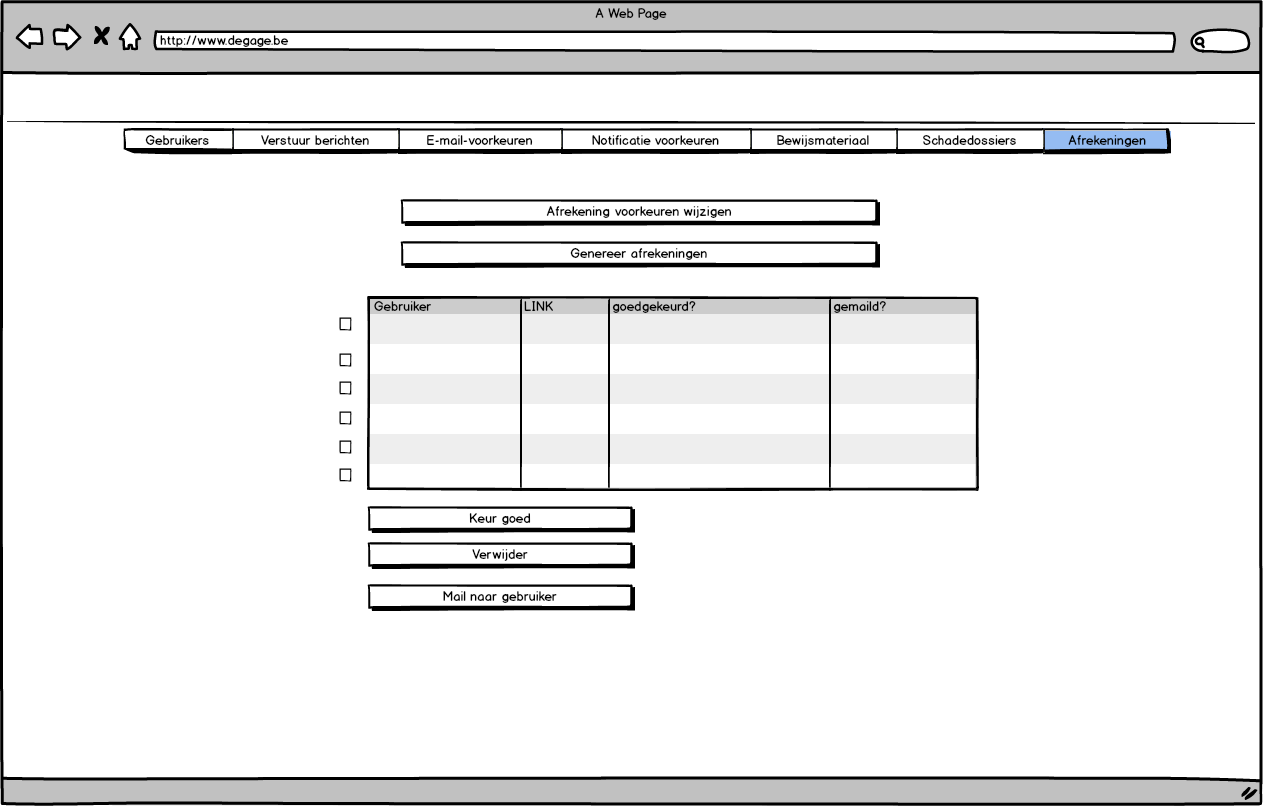
\includegraphics[scale=0.4]{mockups/admin_afrekeningen.png}
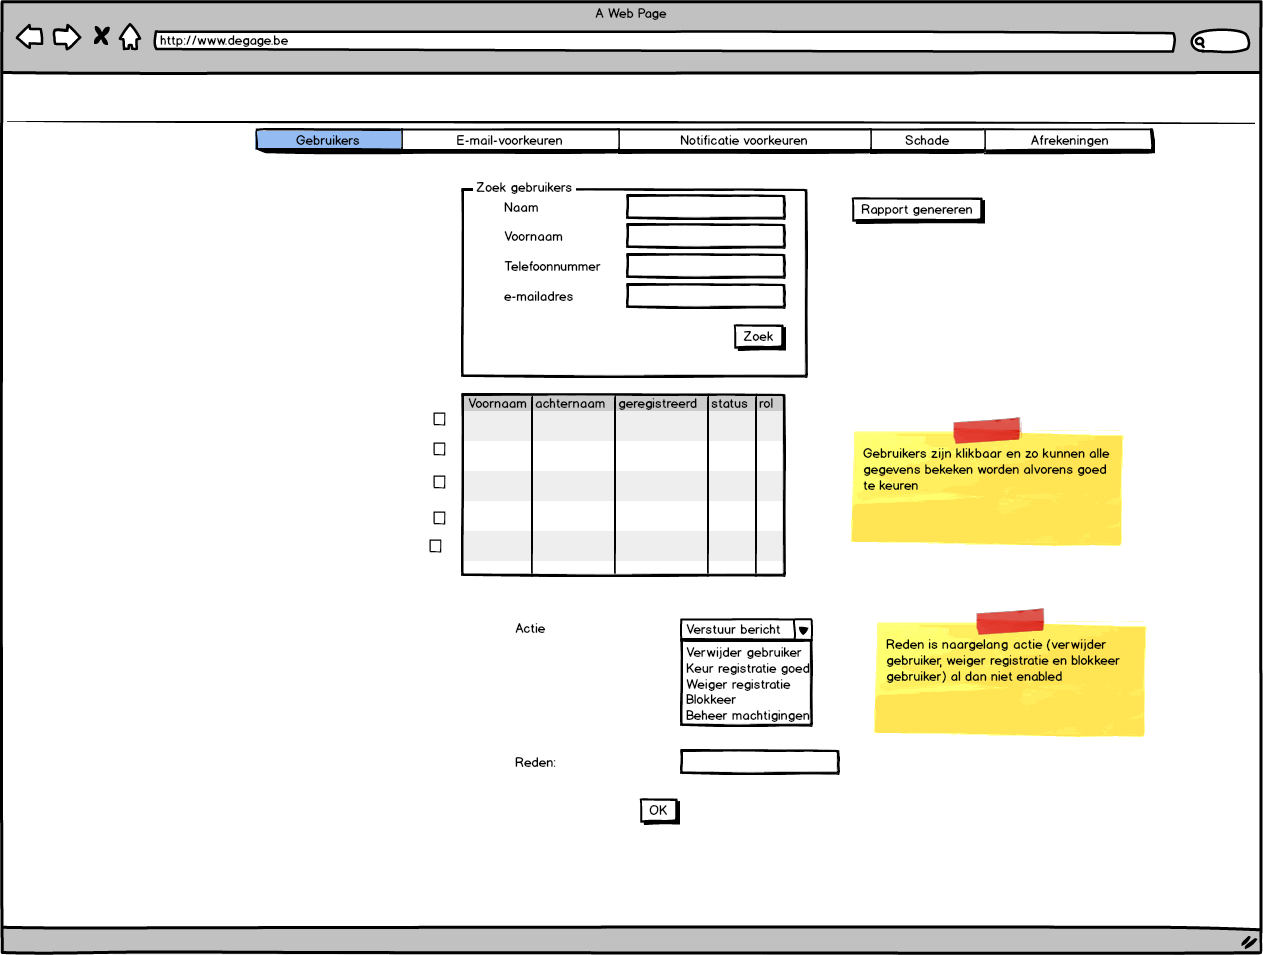
\includegraphics[scale=0.4]{mockups/admin_dashboard_gebruikers.png}
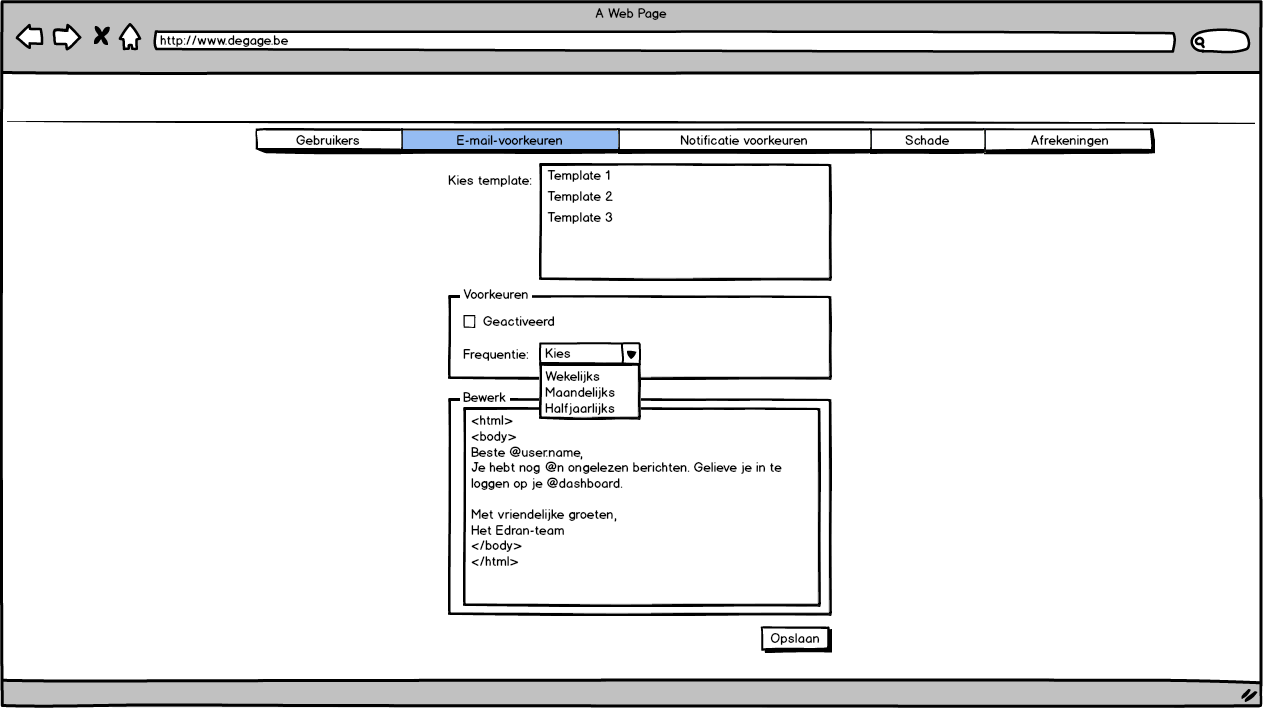
\includegraphics[scale=0.4]{mockups/admin_dashboard_mailvoorkeuren.png}
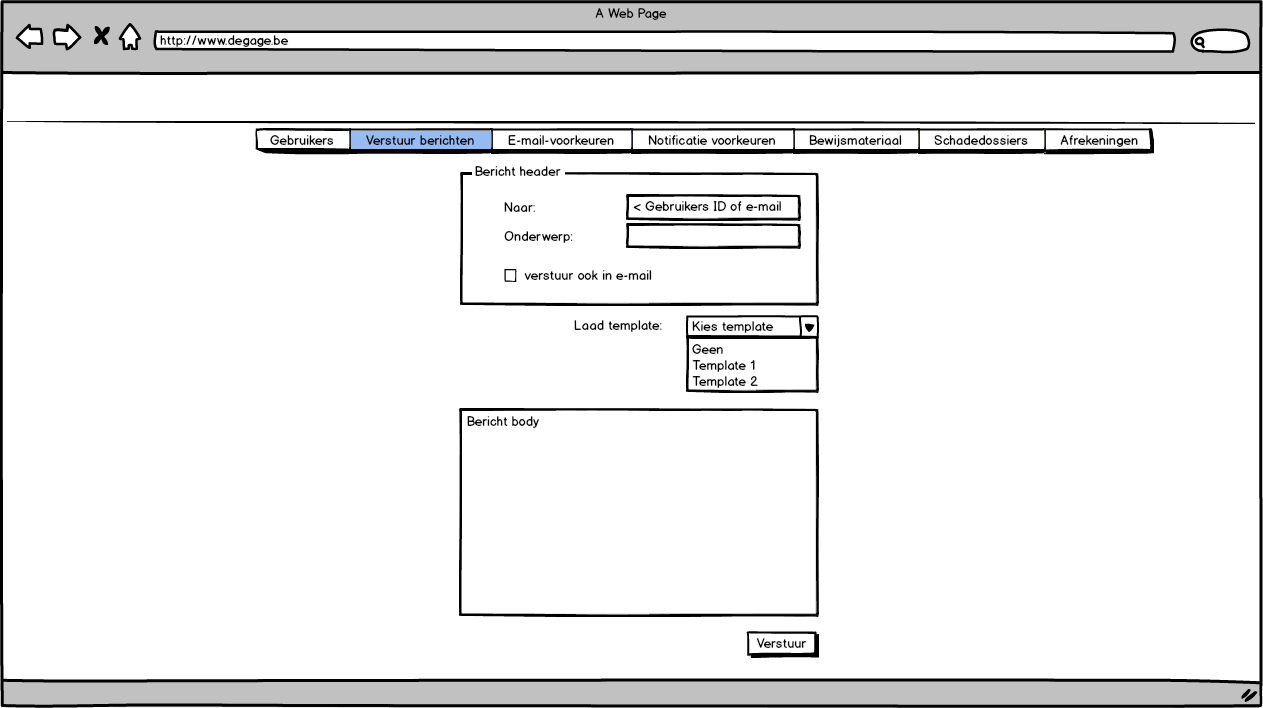
\includegraphics[scale=0.4]{mockups/admin_dashboard_stuur_bericht.png}
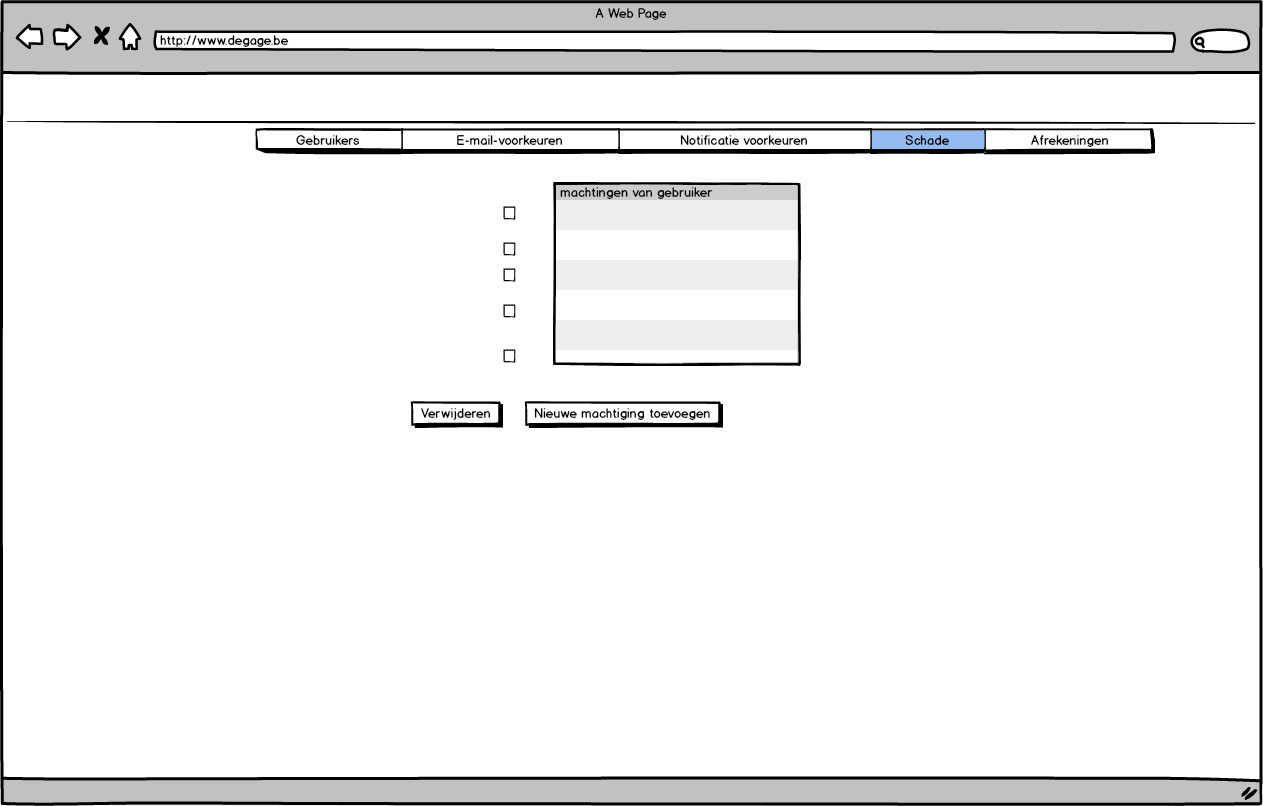
\includegraphics[scale=0.4]{mockups/admin_machtigingentoevoegen.png}
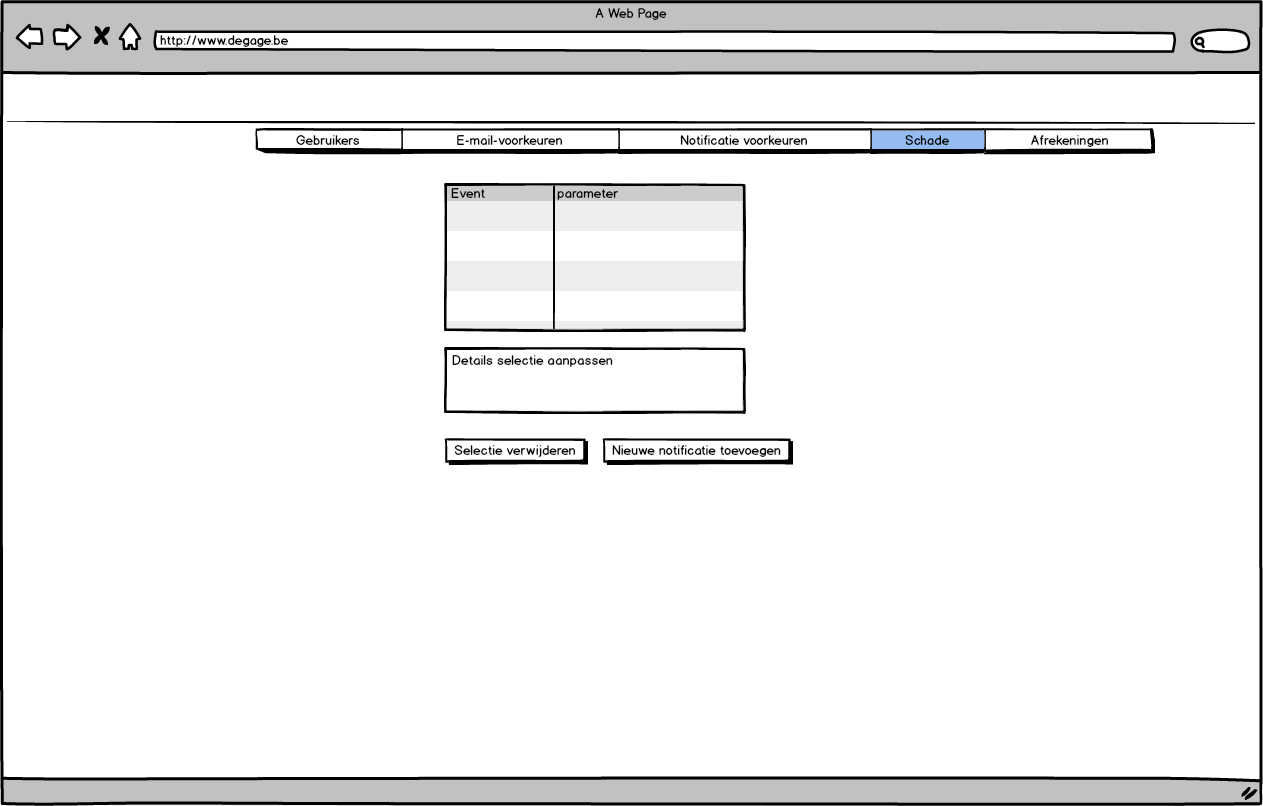
\includegraphics[scale=0.4]{mockups/admin_notificatievoorkeuren.png}
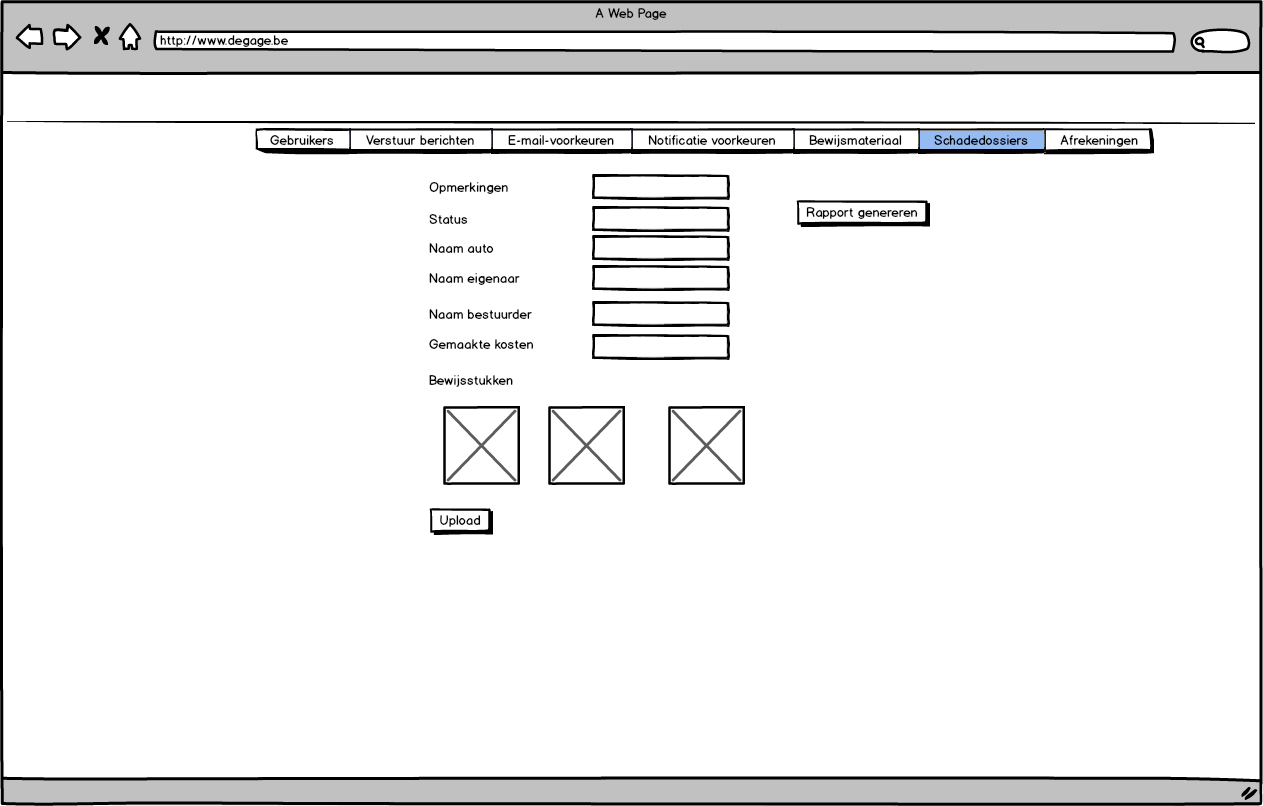
\includegraphics[scale=0.4]{mockups/admin_schadedossiermaken.png}
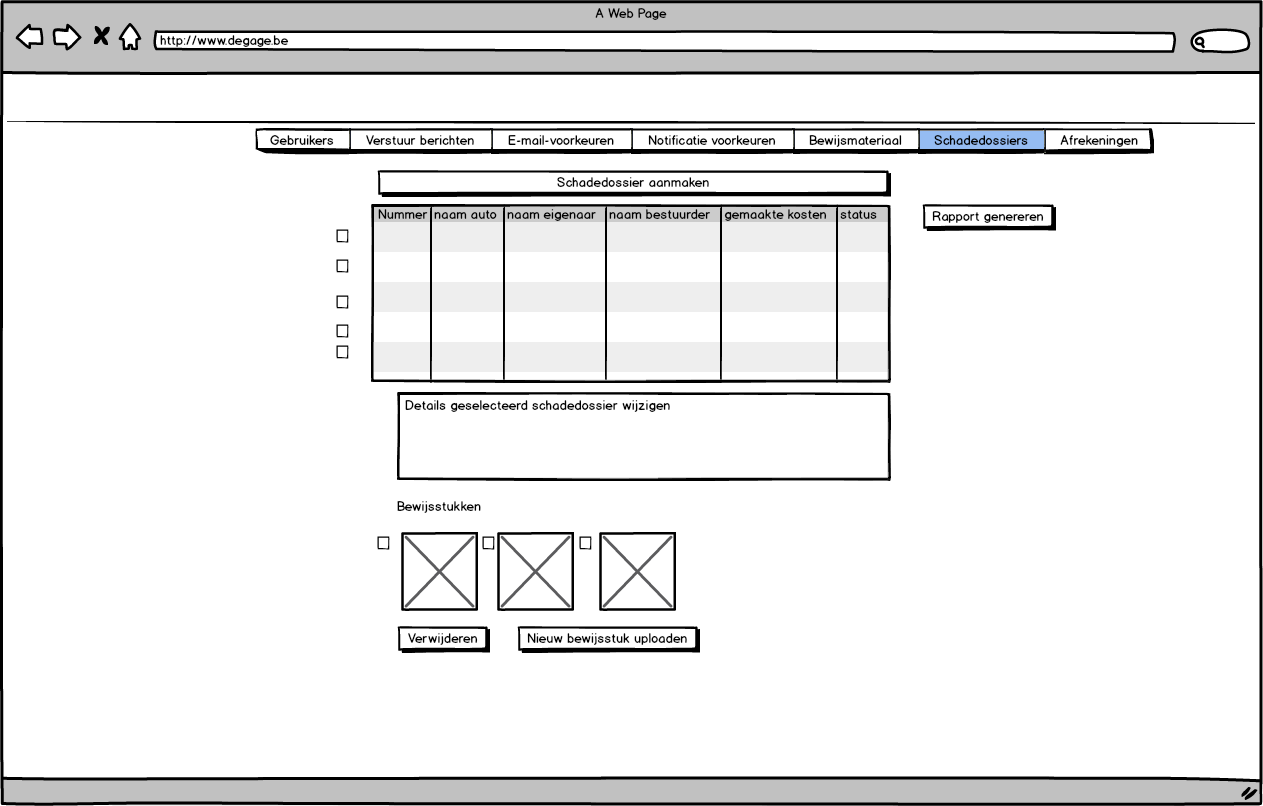
\includegraphics[scale=0.4]{mockups/admin_schadedossiers.png}
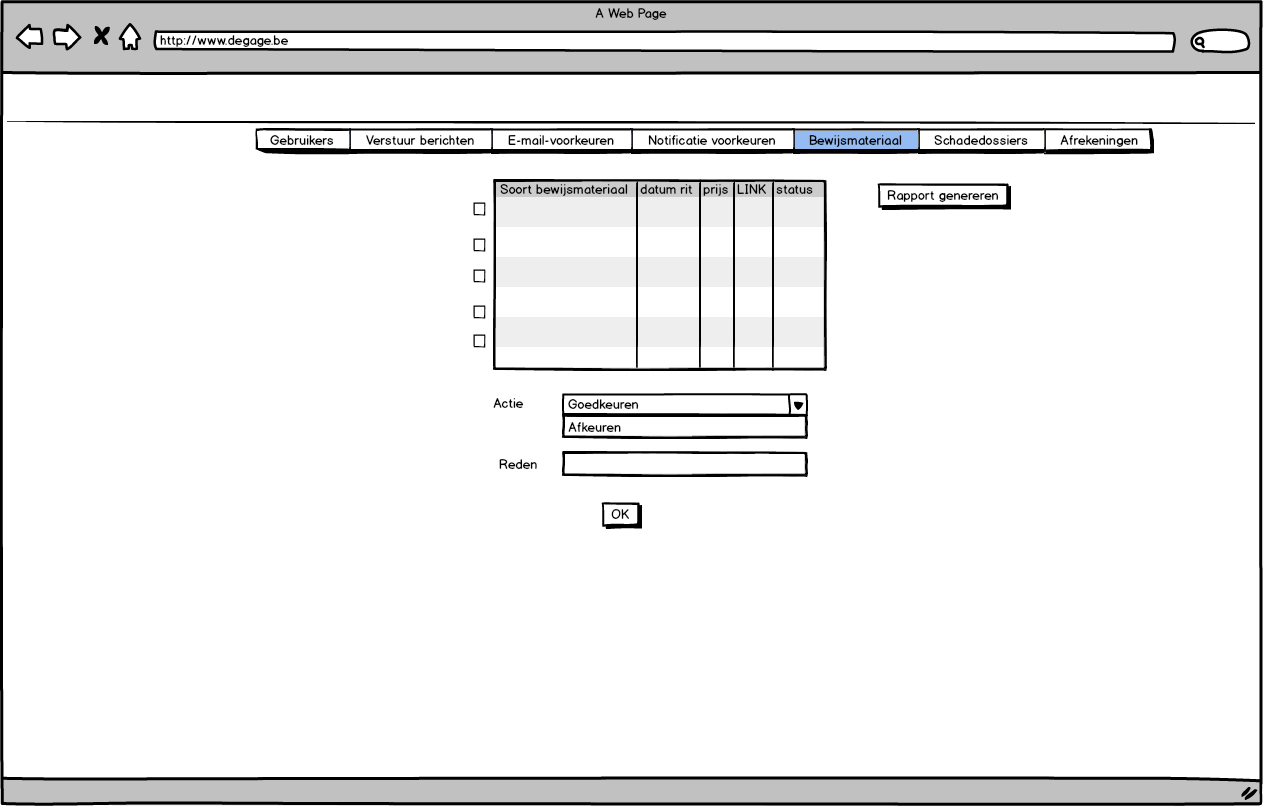
\includegraphics[scale=0.4]{mockups/admin_verifierenbewijsmateriaal.png}
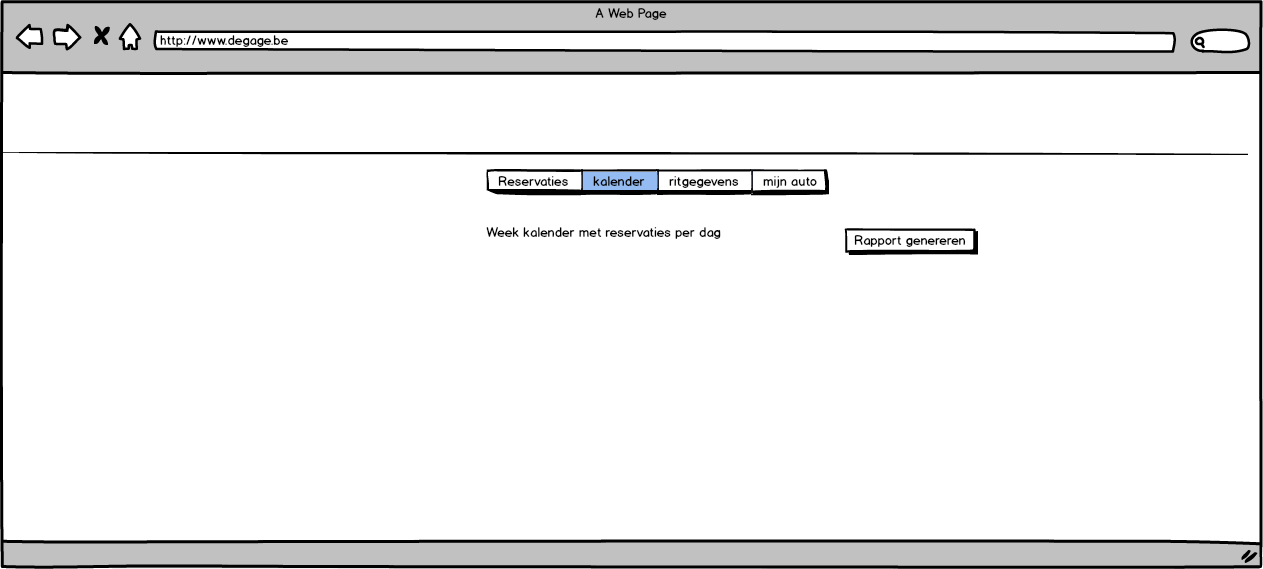
\includegraphics[scale=0.4]{mockups/autobeheer_kalender.png}
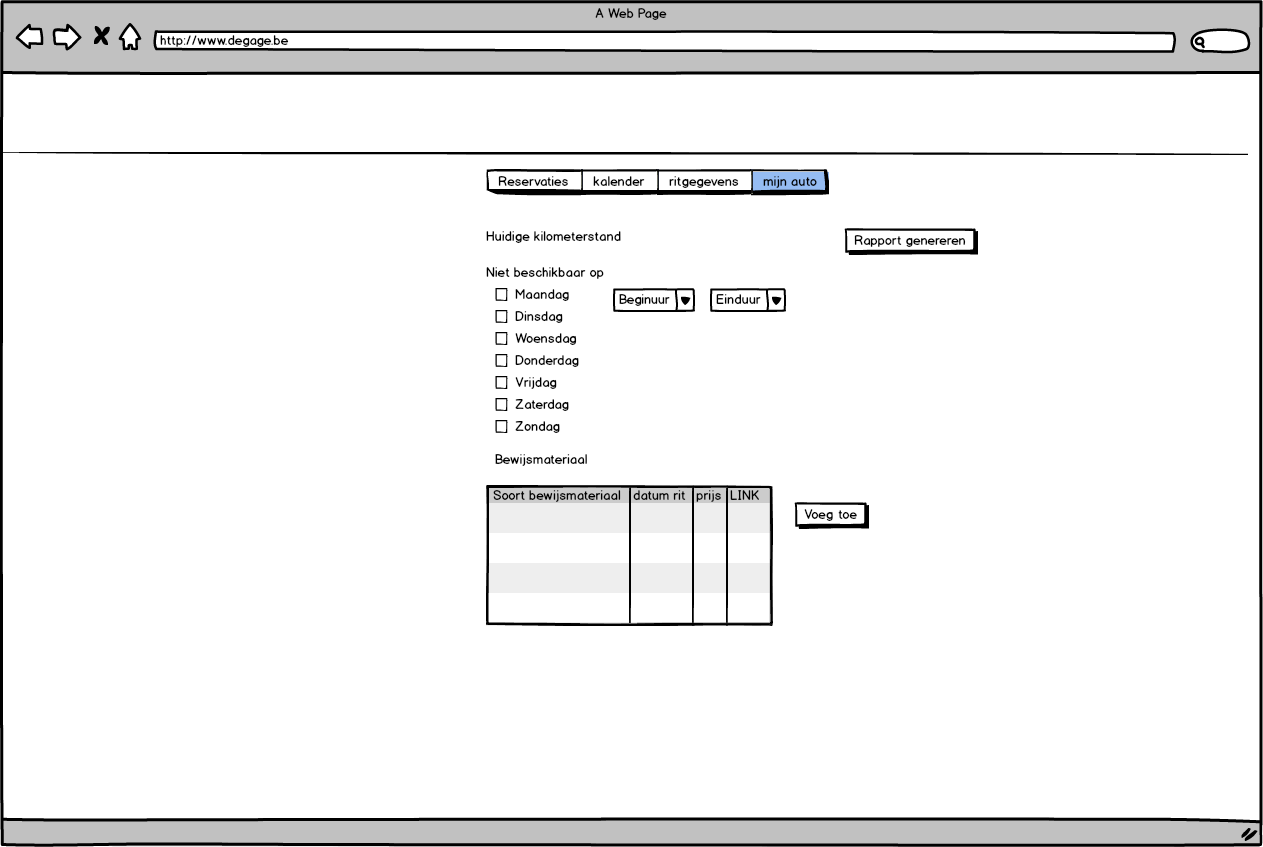
\includegraphics[scale=0.4]{mockups/autobeheer_mijnauto.png}
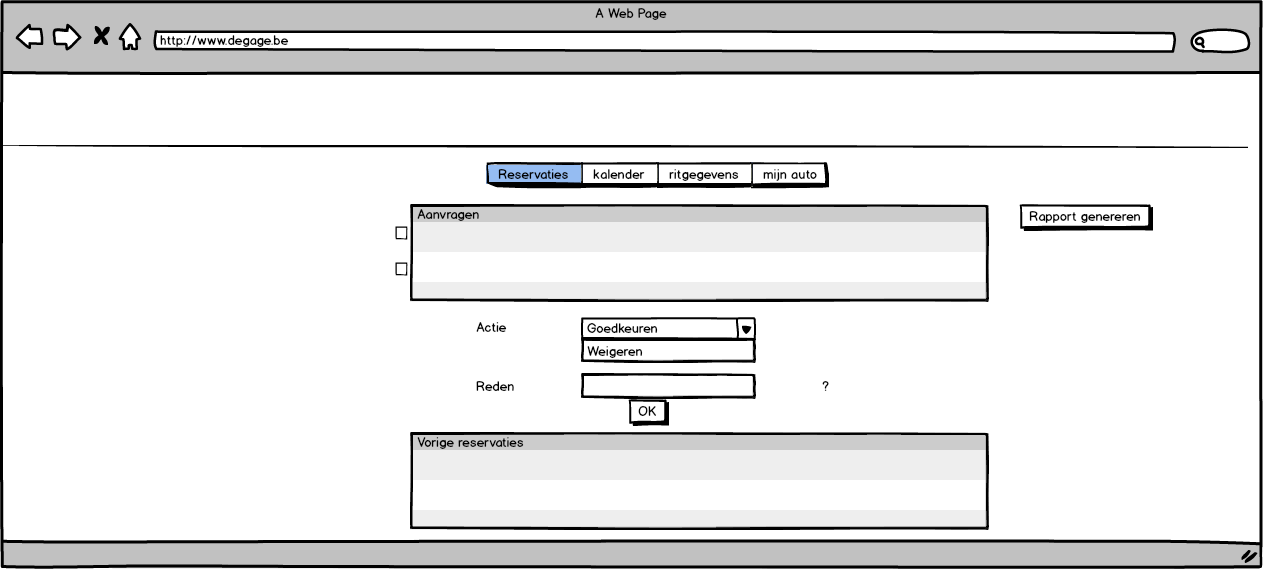
\includegraphics[scale=0.4]{mockups/autobeheer_reservaties.png}
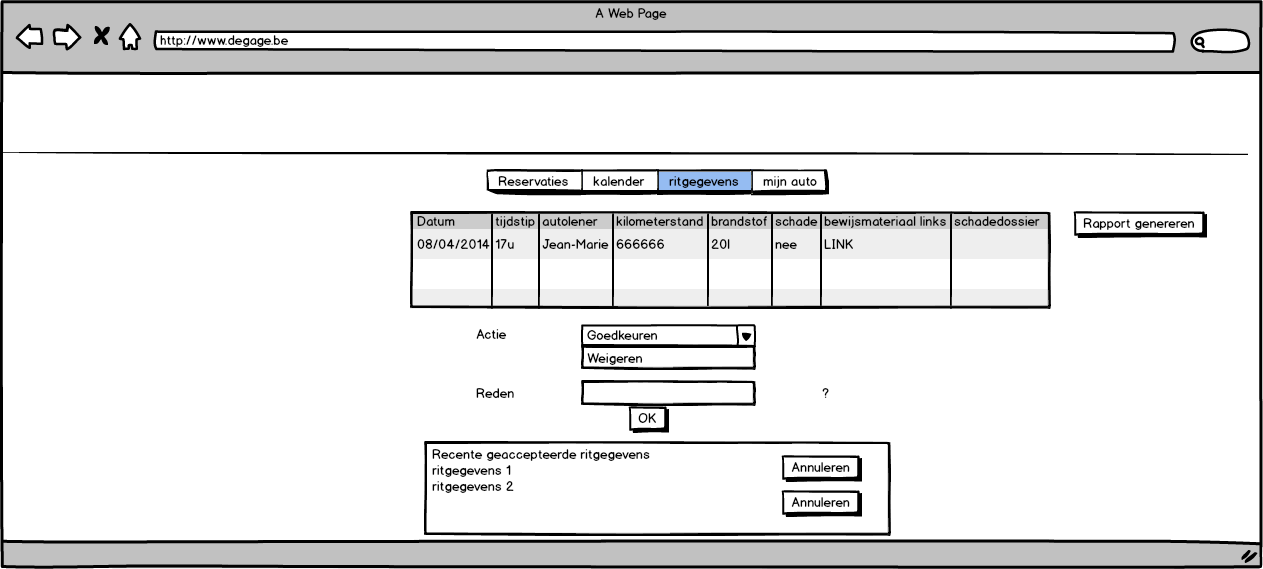
\includegraphics[scale=0.4]{mockups/autobeheer_ritgegevens.png}
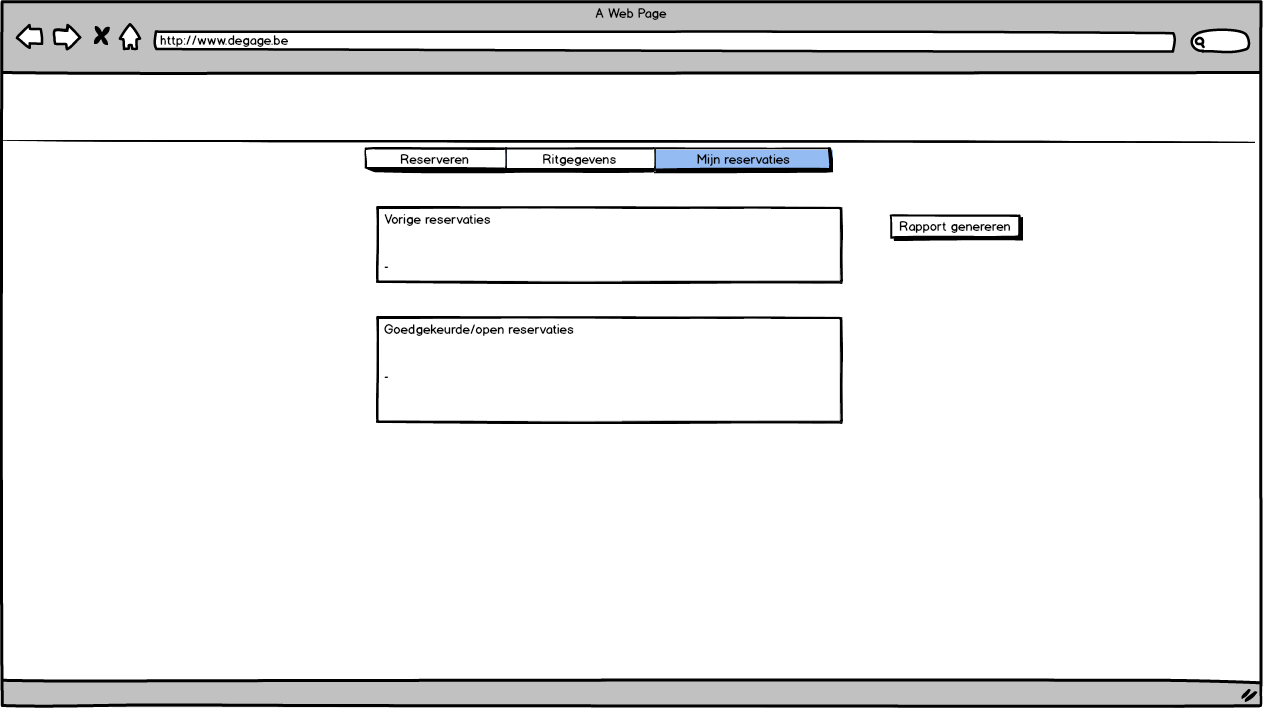
\includegraphics[scale=0.4]{mockups/delen_mijnreservaties.png}
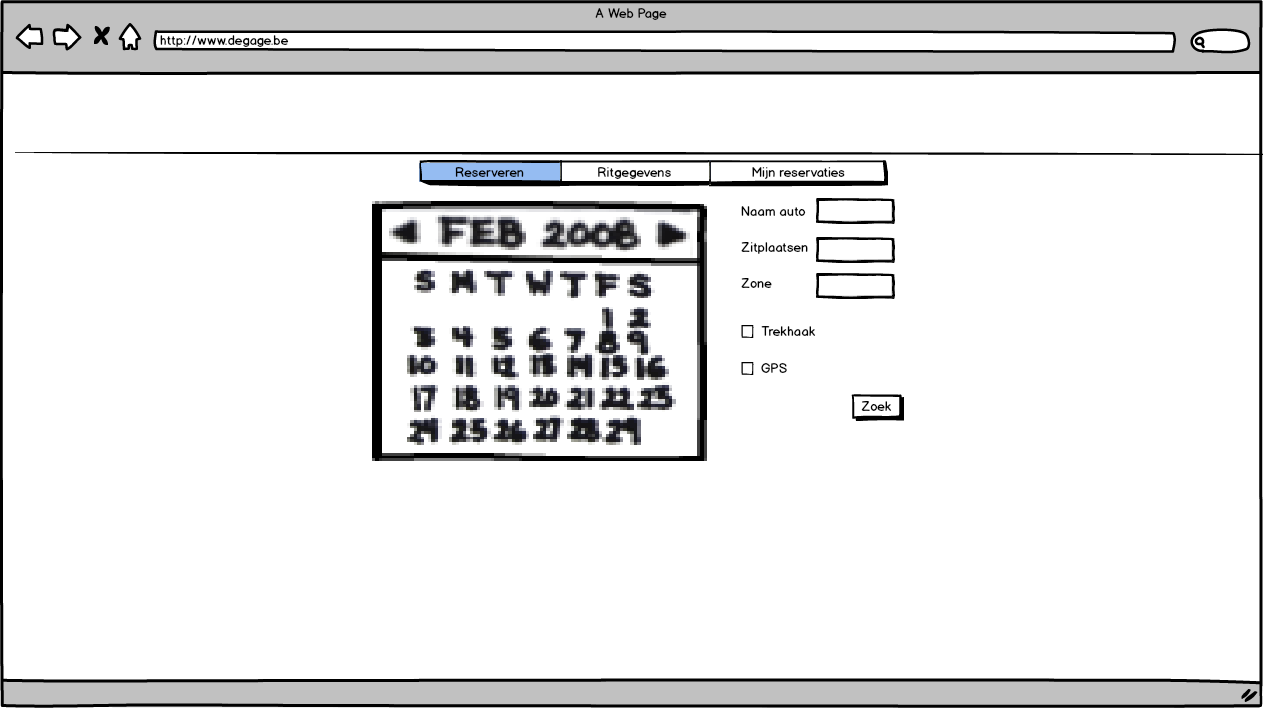
\includegraphics[scale=0.4]{mockups/delen_reserveren.png}
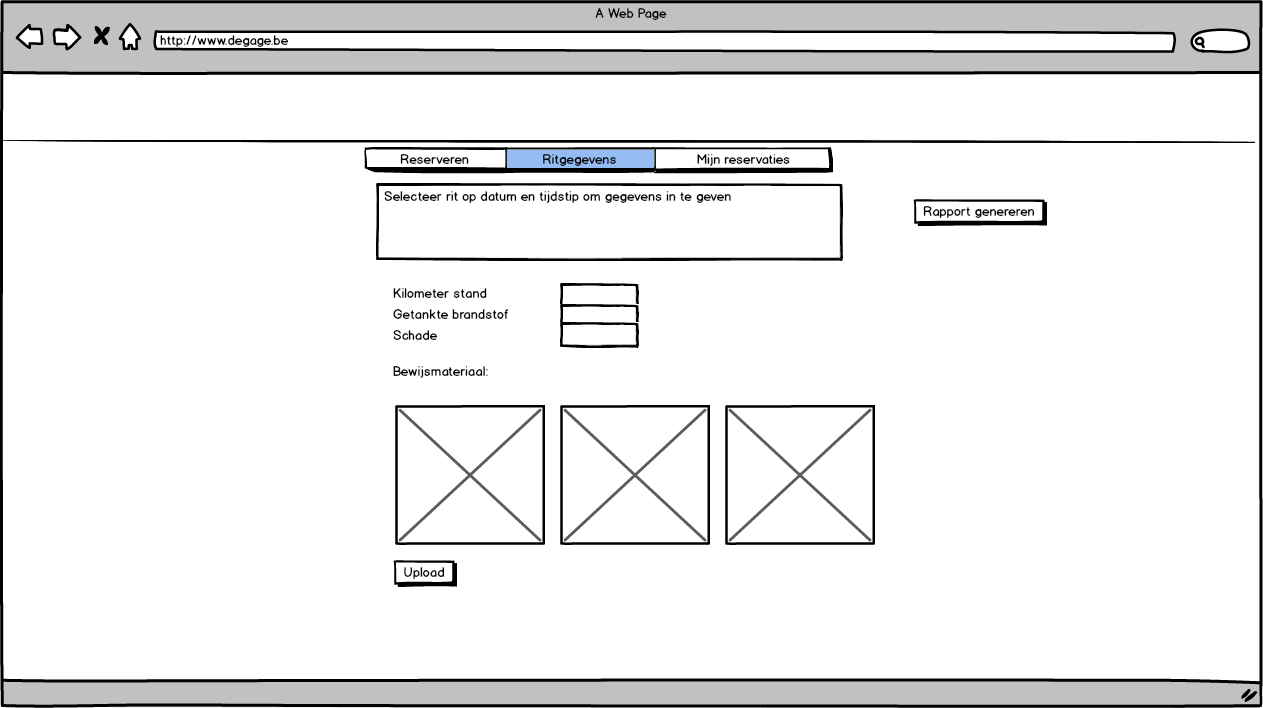
\includegraphics[scale=0.4]{mockups/delen_ritgegevens.png}
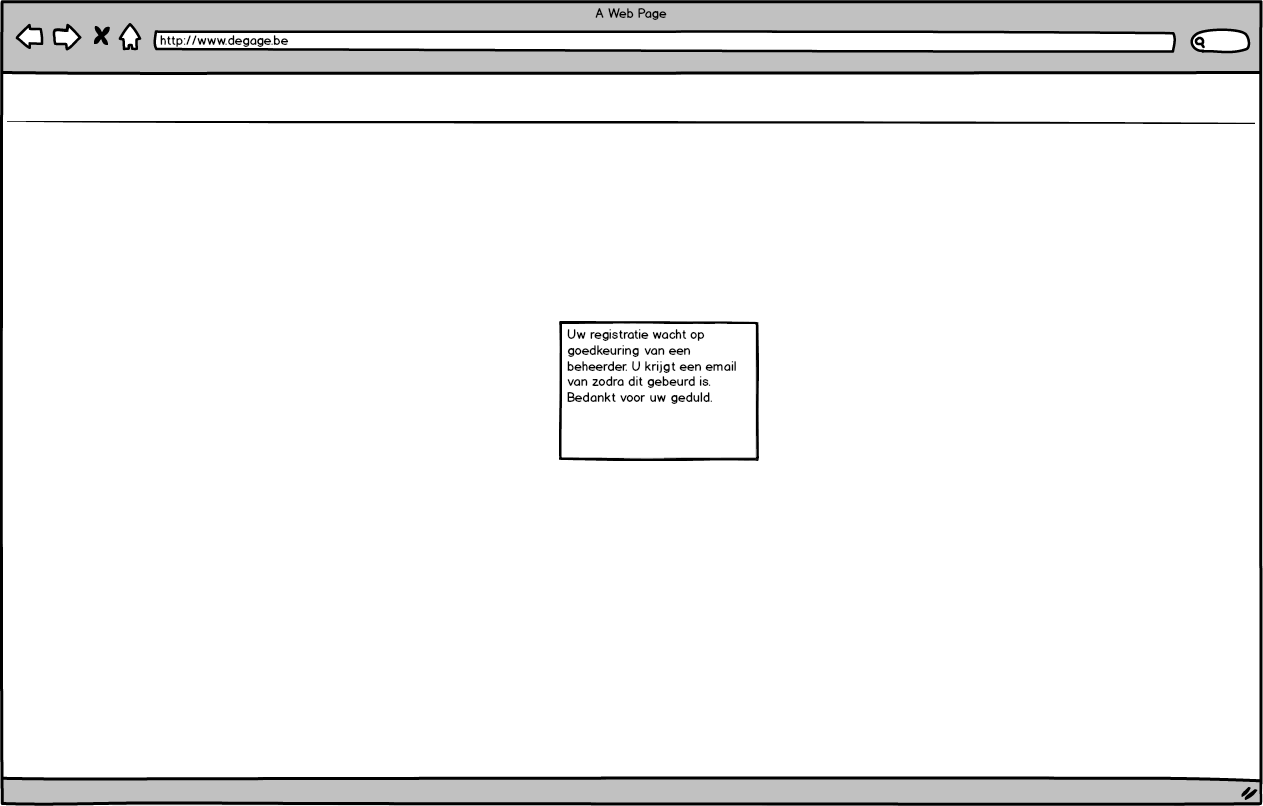
\includegraphics[scale=0.4]{mockups/goedkeuringpending.png}
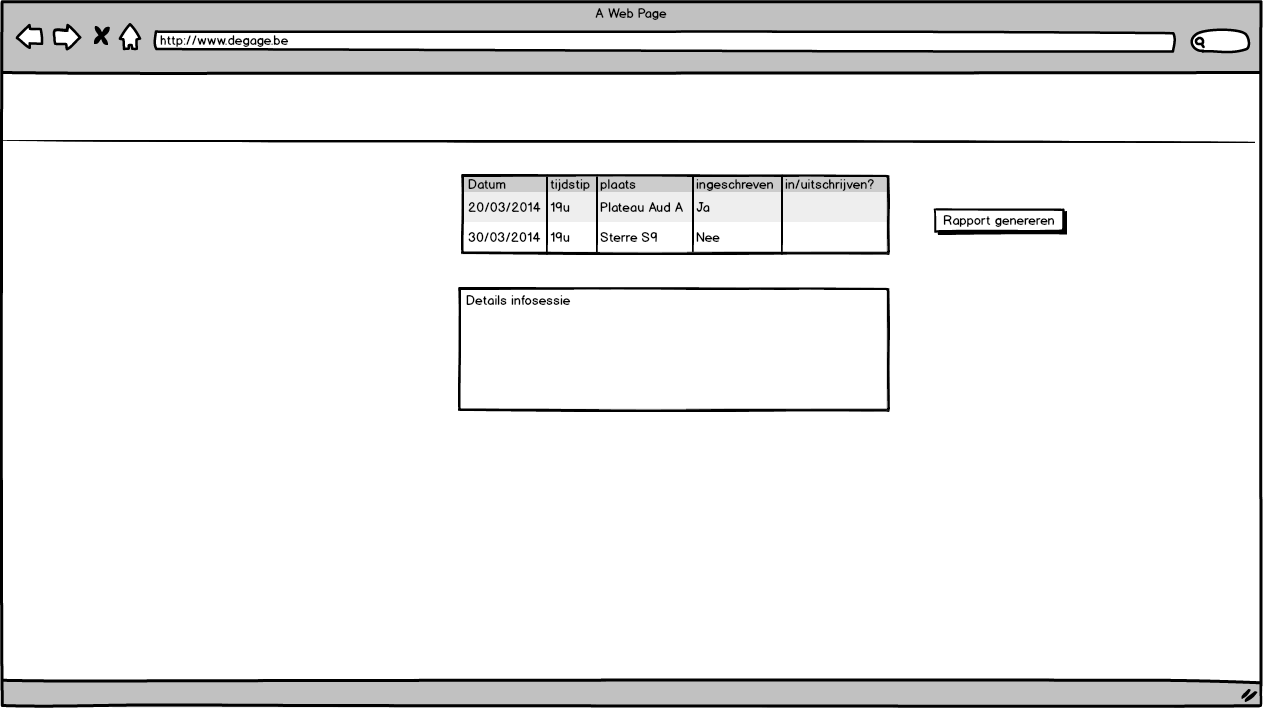
\includegraphics[scale=0.4]{mockups/infosessies_autolener.png}
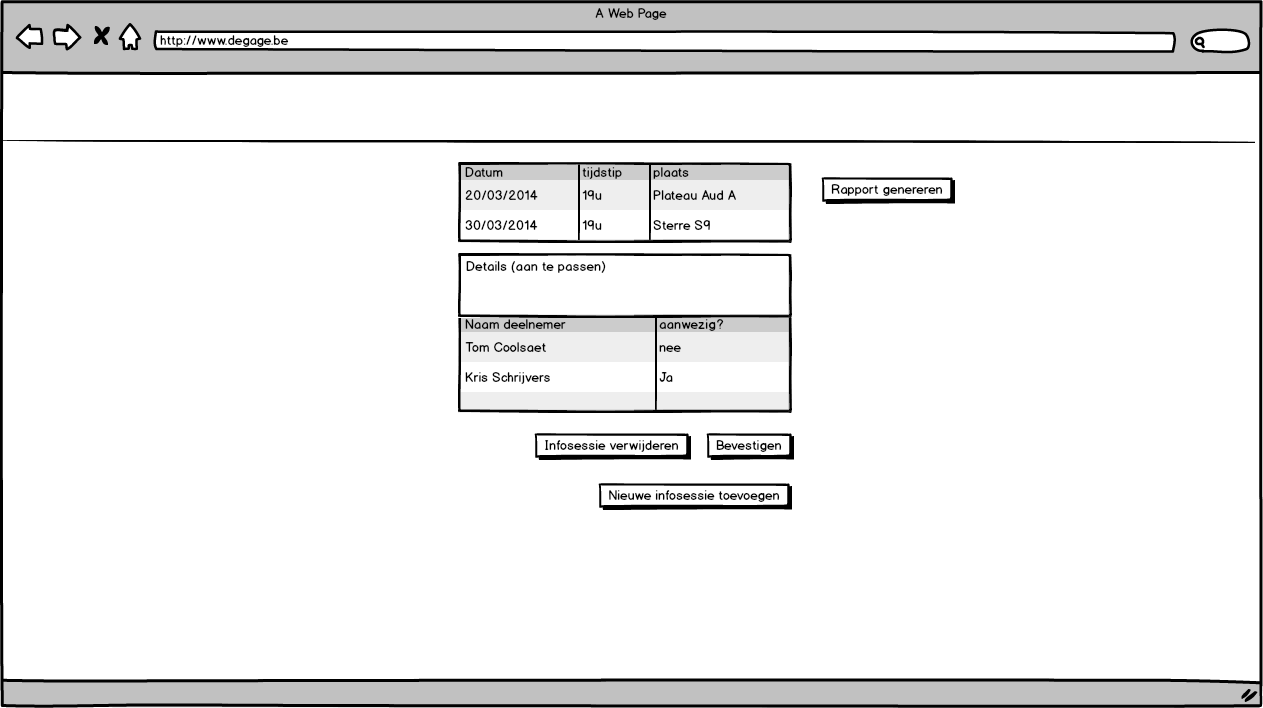
\includegraphics[scale=0.4]{mockups/infosessies_beheerder.png}
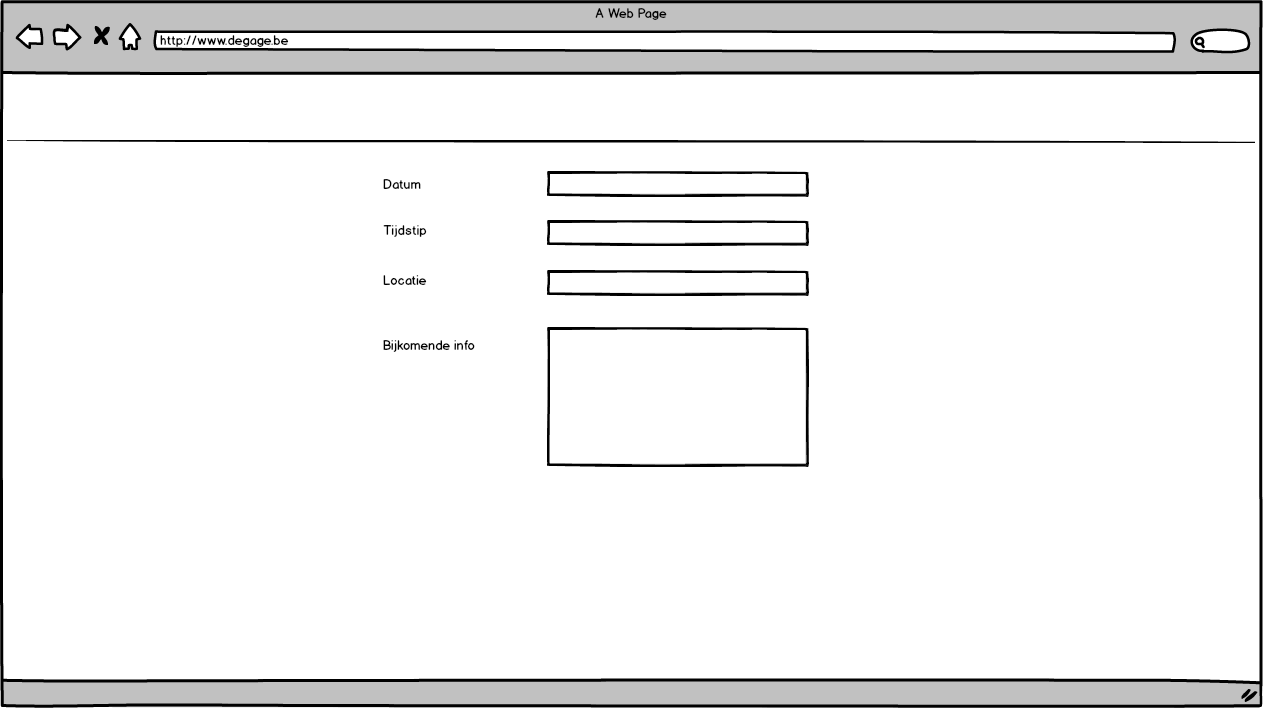
\includegraphics[scale=0.4]{mockups/infosessies_toevoegen.png}
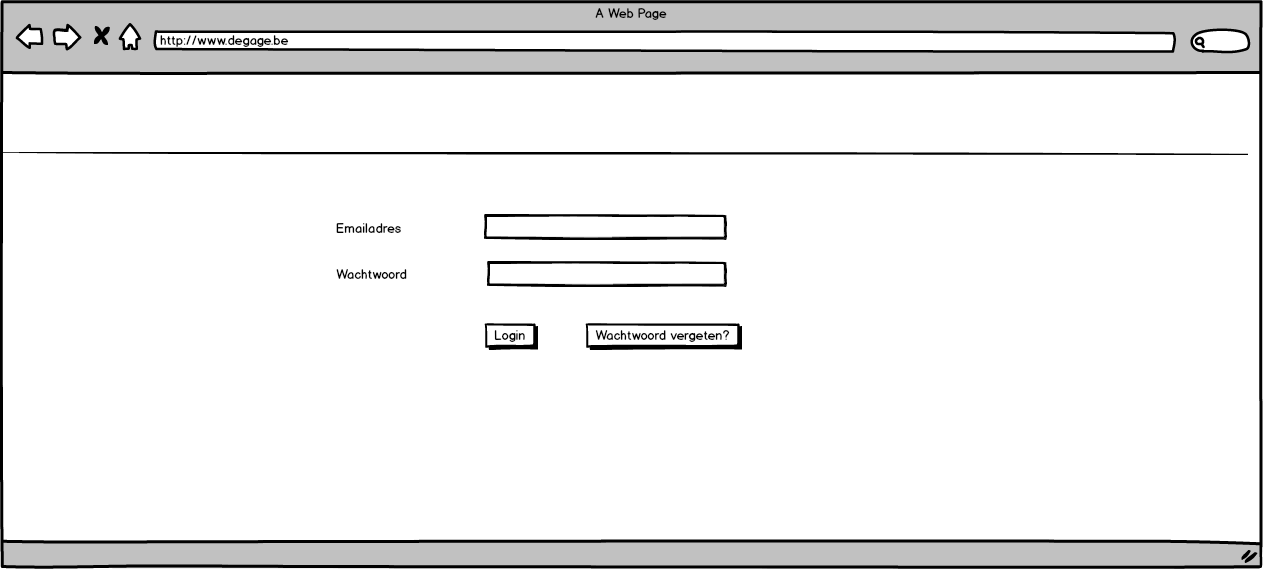
\includegraphics[scale=0.4]{mockups/login.png}
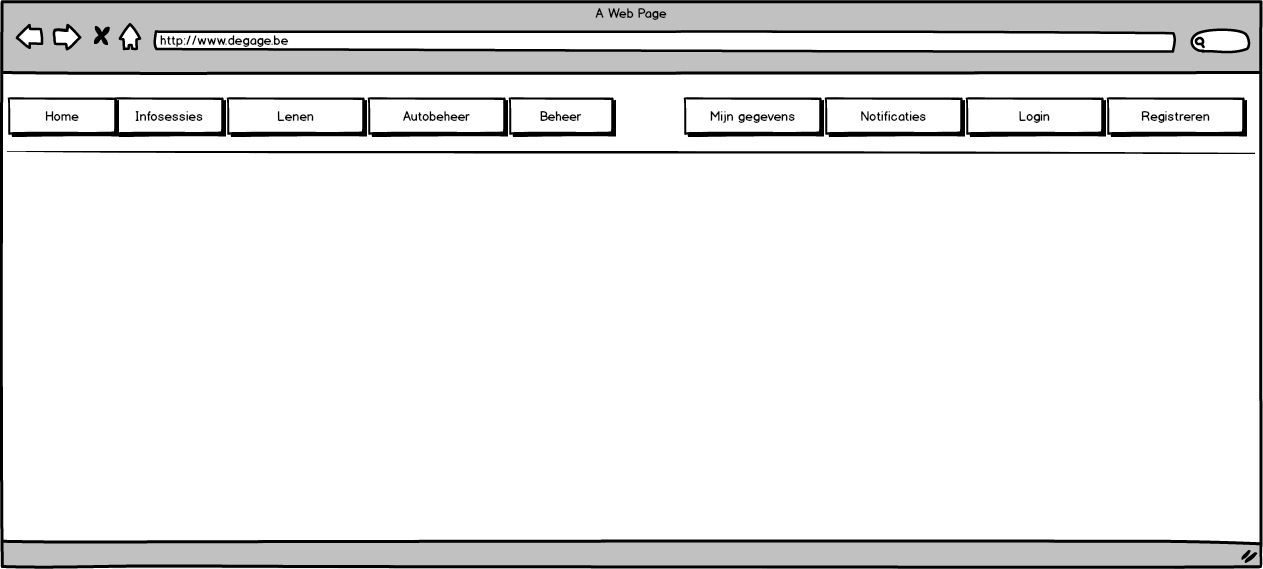
\includegraphics[scale=0.4]{mockups/menu.png}
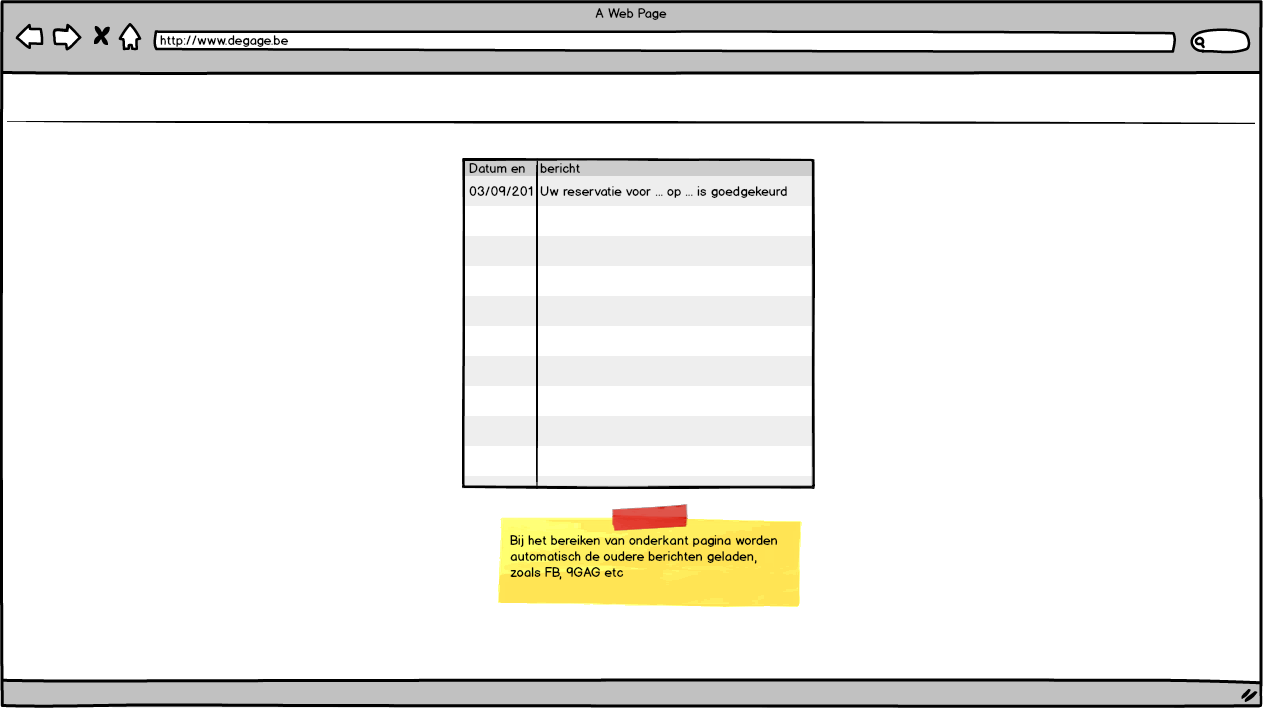
\includegraphics[scale=0.4]{mockups/notificaties.png}
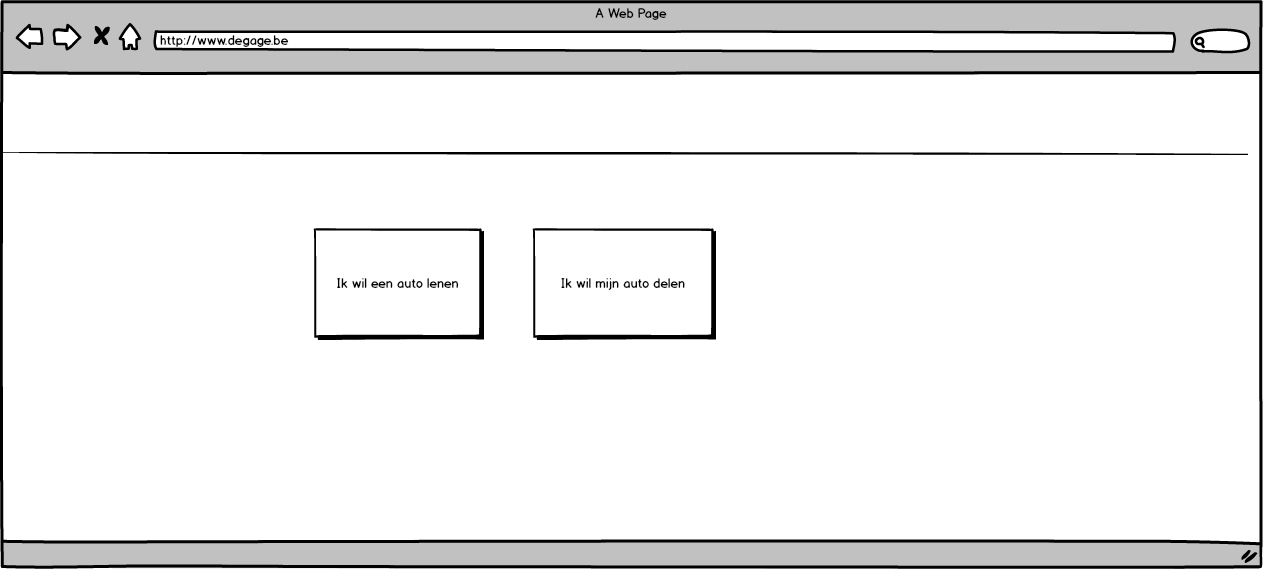
\includegraphics[scale=0.4]{mockups/registratie.png}
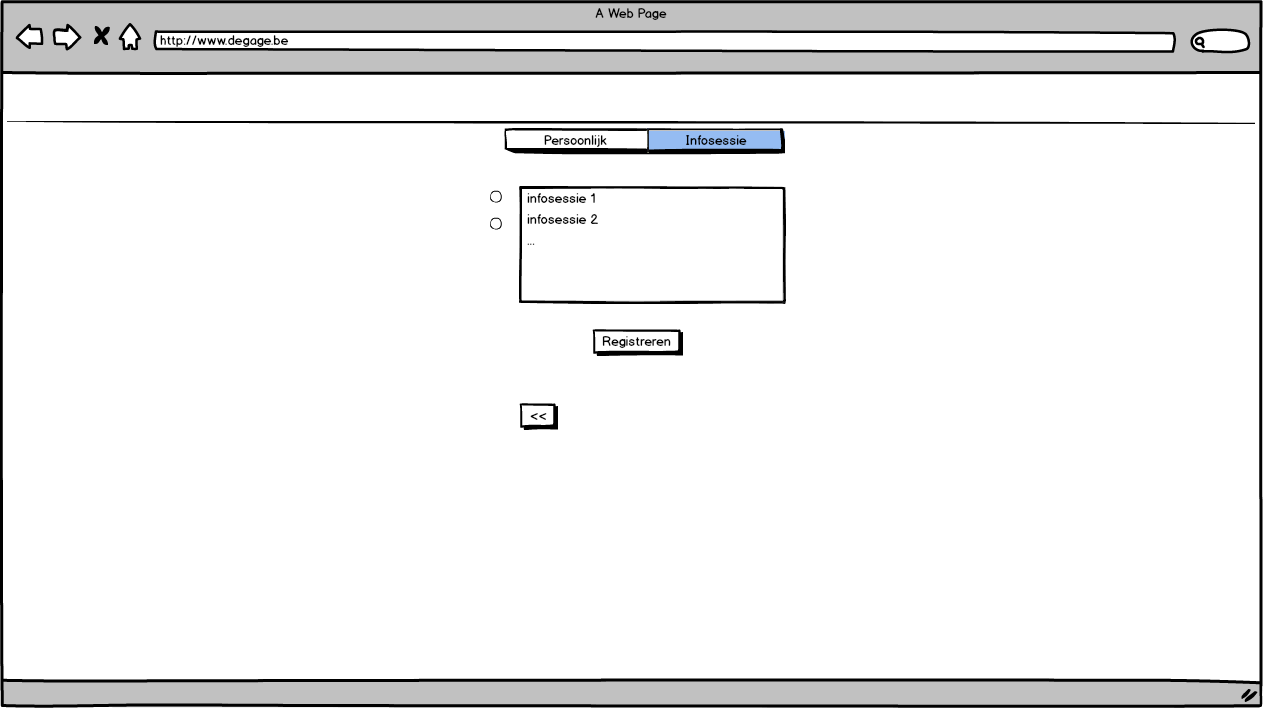
\includegraphics[scale=0.4]{mockups/registratie_autolener_infosessie.png}
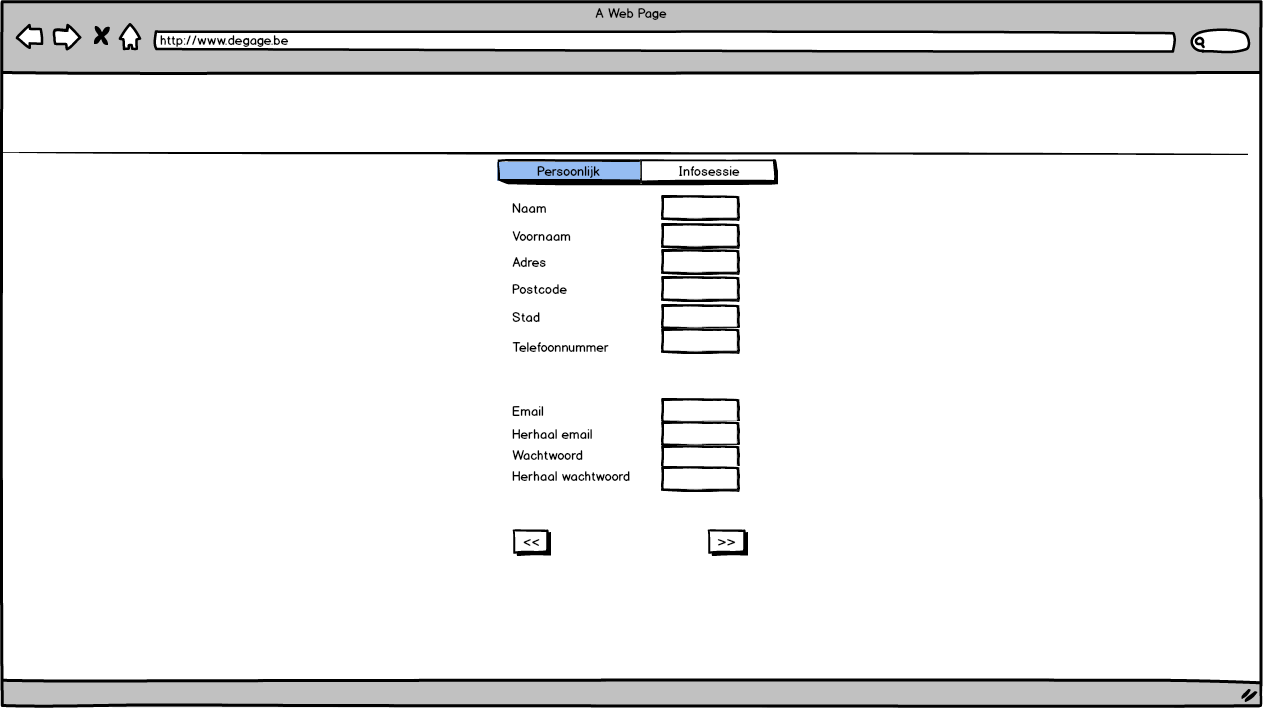
\includegraphics[scale=0.4]{mockups/registratie_autolener_persoonlijk.png}
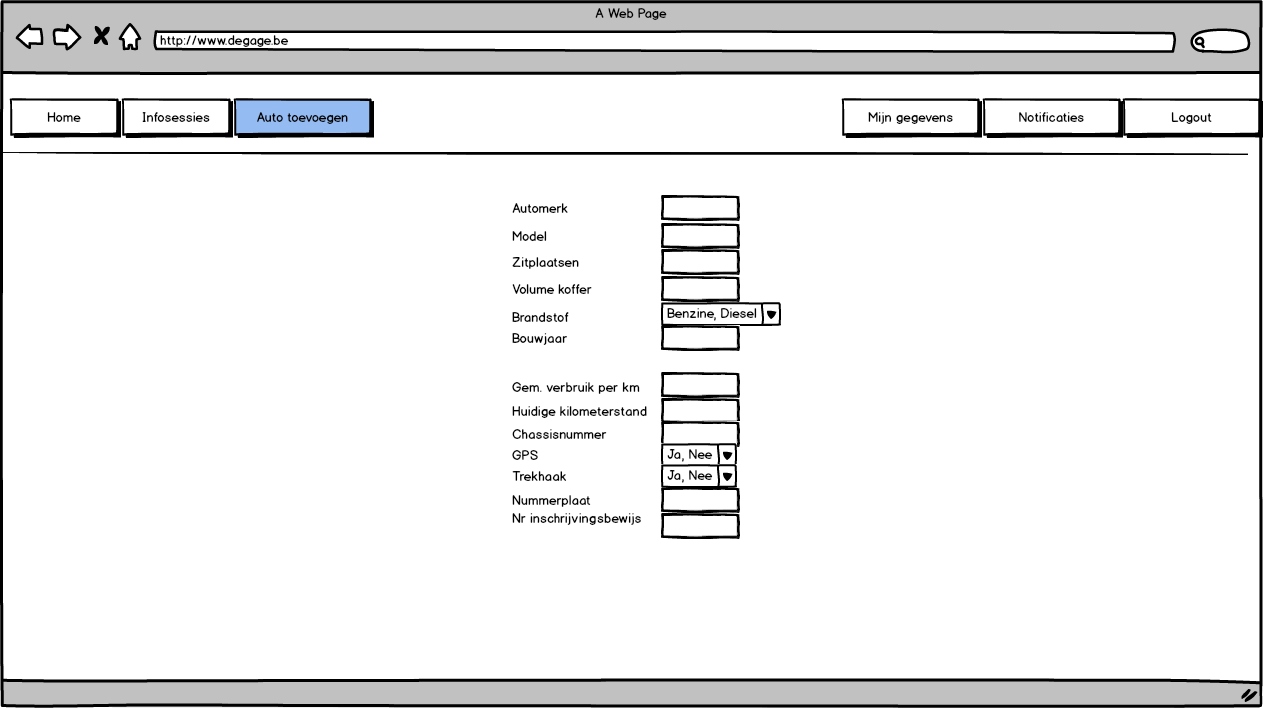
\includegraphics[scale=0.4]{mockups/registratie_eigenaar_auto.png}
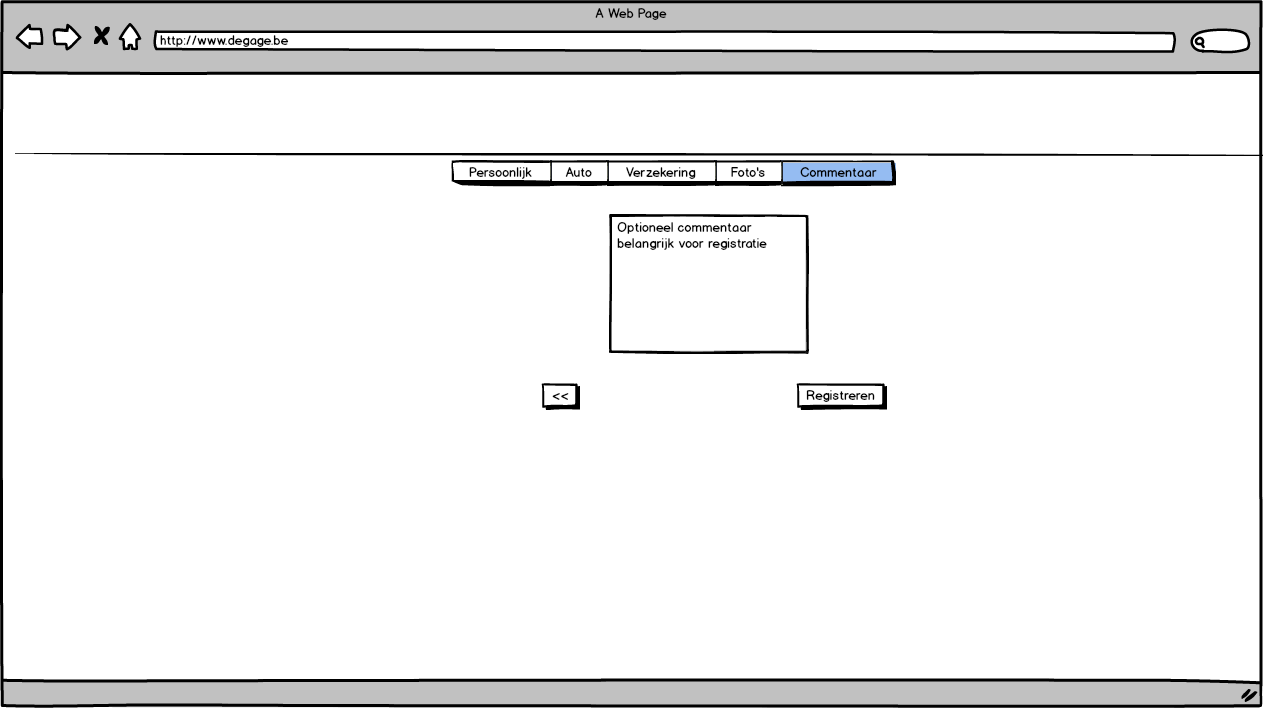
\includegraphics[scale=0.4]{mockups/registratie_eigenaar_commentaar.png}
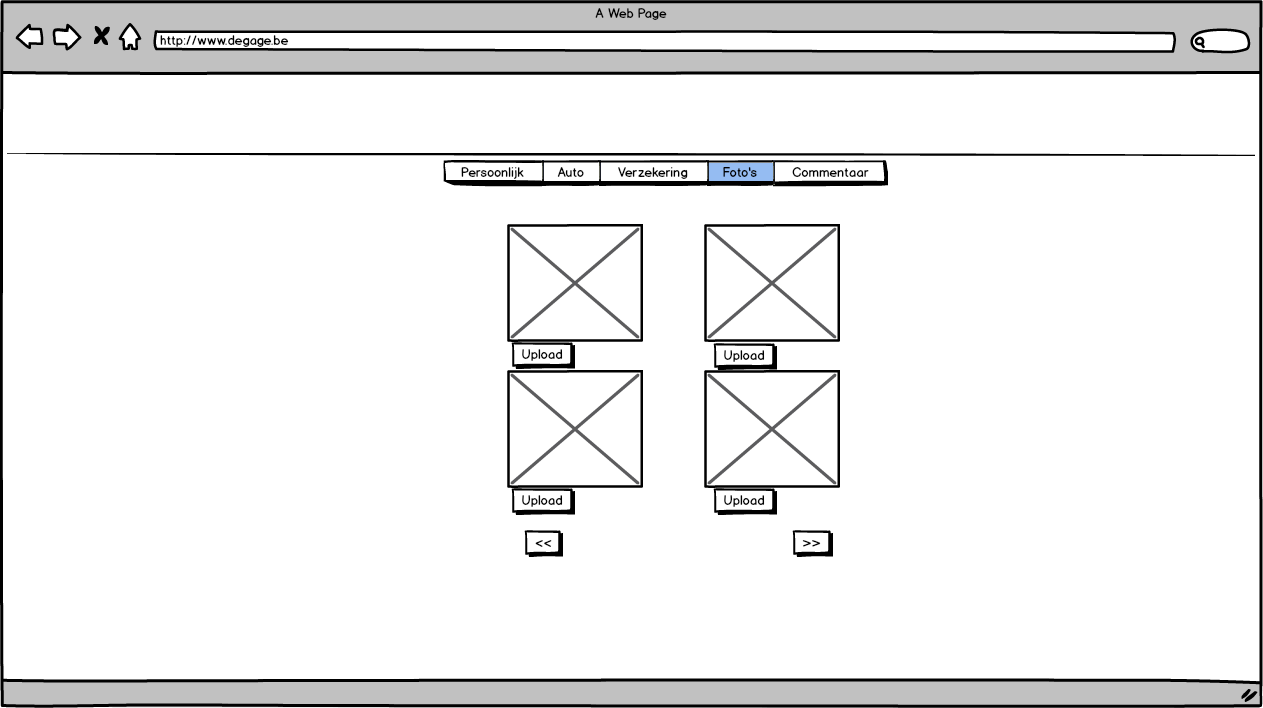
\includegraphics[scale=0.4]{mockups/registratie_eigenaar_fotos.png}
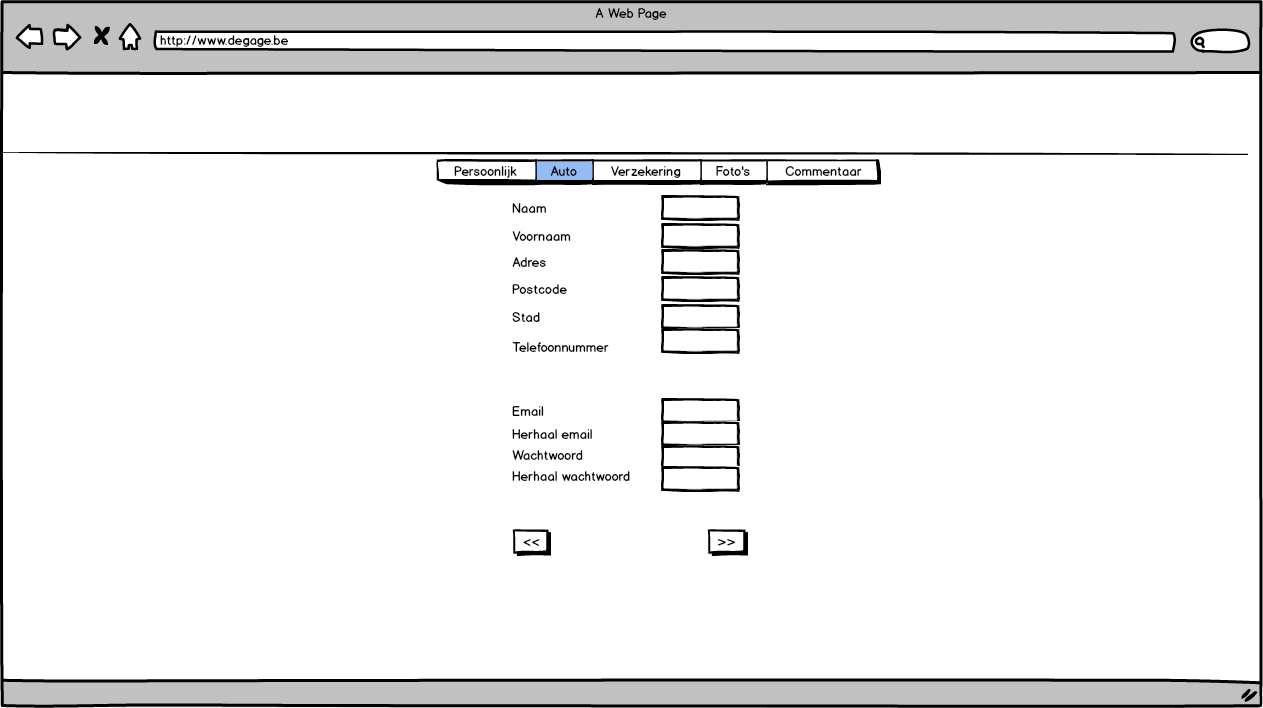
\includegraphics[scale=0.4]{mockups/registratie_eigenaar_persoonlijk.png}
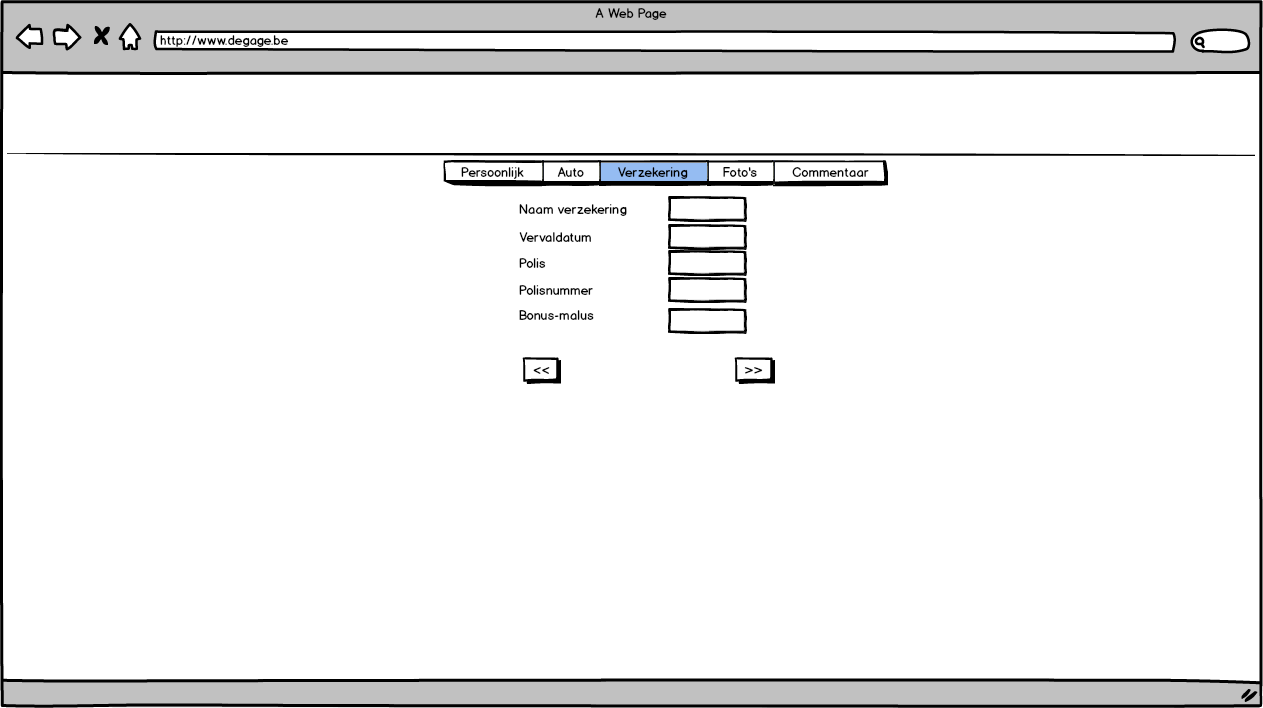
\includegraphics[scale=0.4]{mockups/registratie_eigenaar_verzekering.png}
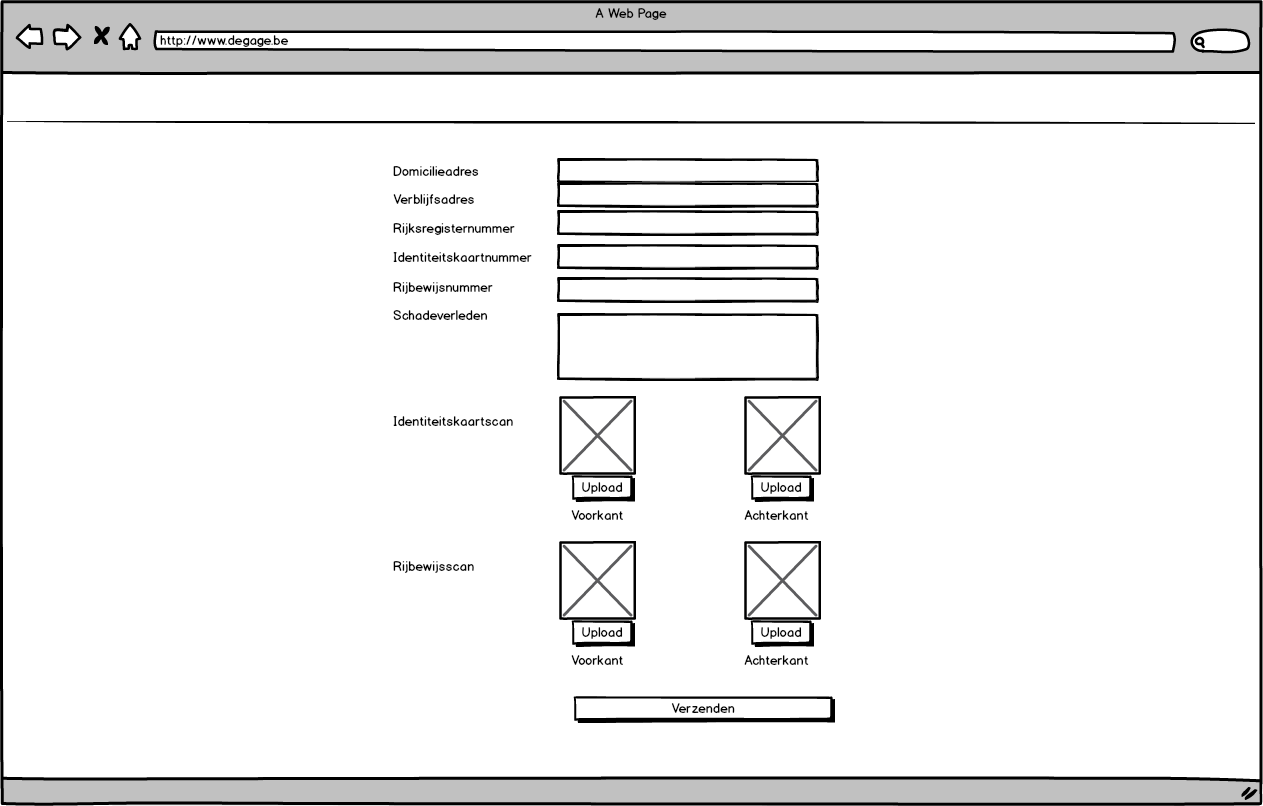
\includegraphics[scale=0.4]{mockups/registratievervolledigen.png}
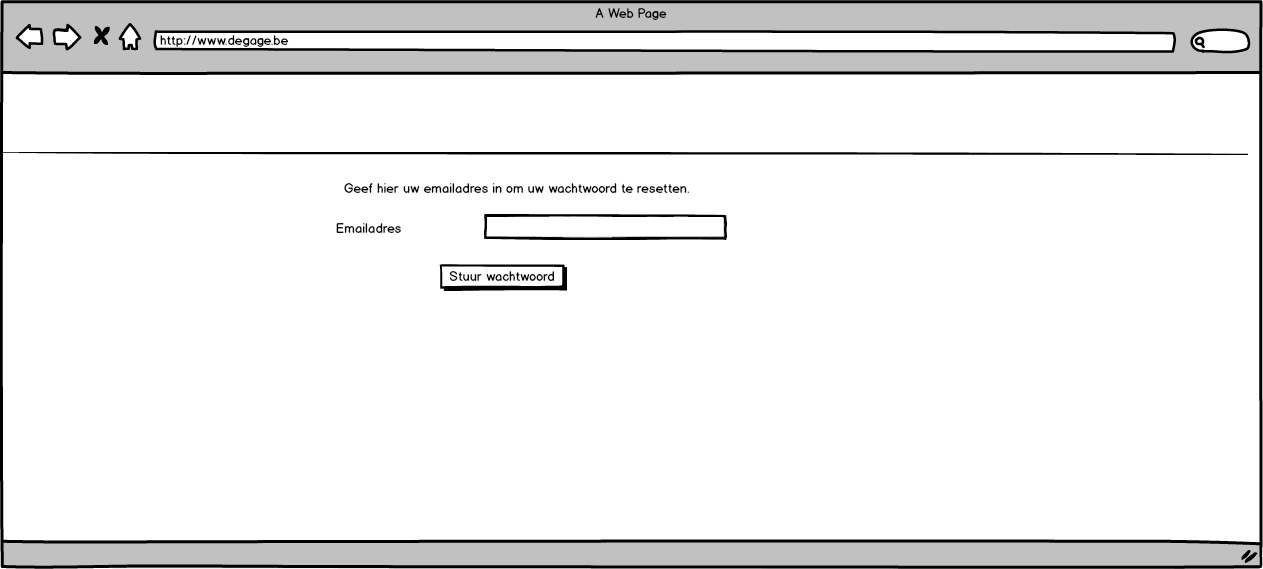
\includegraphics[scale=0.4]{mockups/wachtwoordvergeten.png}
\end{document}